\documentclass[]{dsadokumentation}

% Page breaks before every section (for proofreading)
% \let\oldsection\section
% \renewcommand\section{\cleardoublepage\oldsection}

% Extra packages / definitions
\usepackage{amssymb}
\usepackage{amsthm}
\usepackage{algorithm}
\usepackage[noend]{algpseudocode}
\usepackage{wrapfig}



% Bibliography
\addbibresource{kurs4.2.bib}

% Custom Commands / definitions
\setcounter{chapter}{1}
\newcommand\myacademy{Wolfsberg 2022}

\usepackage{xcolor}
\newcommand\comment[1]{{\color{red} \textbf{#1}}}


\begin{document}

\begin{itemize}
	\item Größere Themen
	\begin{itemize}
		\item Einleitung TN
		\item Schlusswort
		\item Logo
		\item Reihenfolge (alle Sections entweder mit keiner Subsection oder min. 3 subsections)
		\item Alle Sätze noch einmal durchlesen und holprige Sätze verbessern.
	\end{itemize}
	\item Kleinere Themen
	\begin{itemize}
		\item Alle Einheiten nicht kursiv
		\item Alle Formeln durchschauen, ob sie korrekt formatiert sind.
		\item Alle Absätze müssen mindestens zwei Sätze haben.
		\item Alle Posterthemen: Autor*innennamen. Posterautor*in dahinter in Klammern.
		\item Vereinheitlichen: Subsections vs Paragraphs (z.B. \enquote{Algorithus von Siddon})
		\item Alle Abbildungen aussagekräftige Bildunterschriften (Bild nur beschreiben, Interpretation im Text).
		\item Checken, dass alle Abbildungen im Text referenziert sind und ggf referenzieren.
		\item In Formeln kein \verb|,| sondern \verb|.| für Kommazahlen verwenden
		\item Gleichungen müssen in Satz eingebettet sein und ggf am Ende einen Punkt haben.
		\item Alle Gleichungen mit Nummern (z.B. mit \verb|equation| oder \verb|align|).
	\end{itemize}
	\item KL
	\begin{itemize}
		\item (Einleitung KL)
	\end{itemize}
\end{itemize}

\cleardoublepage

\tableofcontents

\kurs{Die Theorie der Information}{Wie aus Daten Bilder werden}{k4.2/kurslogo.pdf}

\section{Git}
\sectionauthor{Jonas Fiedler, (Clemens Ljungh)}

Mit der Versionsmanagement-Software Git kann Kooperation zwischen mehreren Programmierern ermöglicht werden. Git beschäftigt sich hauptsächlich mit dem Verwalten von Versionen des Codes und der Zusammenführung von Code Änderungen. Dafür erstellt Git einen Versionsverlauf, welcher es ermöglicht, Versionen des Codes zurückrollen um Bugs zu identifizieren und das Nachverfolgen von Code-Änderungen von wichtigen Updates zu ermöglichen. Dabei wird zwischen lokaler Dateispeicherung und Speicherung im serverseitigen Bereich unterschieden. Der Server ermöglicht den Nutzern, Code herunterzuladen, ihn zu bearbeiten und letztendlich in überarbeiteter Version wieder an den Server zu übermitteln, wo dieser dann mit anderen Nutzern ausgetauscht werden kann.

Generell ist es in Git möglich verschiedene Versionsstränge (Branches) aufzubauen. Diese Branches ermöglichen die Modifikation an verschiedenen Bereichen und ein strukturierte Entwicklung von Features. In diesen Branches können somit bspw. Bugs unabhängig gelöst werden und neue Funktionen getestet sowie implementiert werden. Sobald diese ordnungsgemäß funktionieren, werden sie auf den nächst höheren Branch, eine in der Hierarchie übergeordnete Ebene, geschoben (Merge) und somit mit dem Rest des Codes wieder vereint.

In Git gibt es verschiedene Stadien, der \enquote{Codeverarbeitung} um eine Codeversion zu speichern. Dabei beschreibt \verb|git add| den Vorgang wo die Datei von dem Working-Directory (lokal), in die Staging Area (auch lokal) verschoben wird. Der wichtigste Befehl in Git ist \verb|git commit|, dieser hält den aktuellen Zustand des gesamten Projektes fest und speichert diesen im Localrepo. Danach ermöglicht \verb|git push| das Übertragen des Codes an den Server. Der umgekehrte Schritt dazu ist \verb|git pull|. Dies lädt die aktuellste Version des Projektes vom Remoterepo in das Localrepo des Users.

Aufgrund der diversen Verwaltungsoptionen und der Möglichkeit kollaborativ in Git zu arbeiten, wird dieses Tool von vielen Software-Developern, sowie Unternehmen verwendet.

\section{Programmierparadigmen}
\sectionauthor{Alexander Gitnik, Clemens Ljungh, (Jonas Fiedler, Aaron Gschwendt)}
\subsection{Objektorientierte Programmierung}
Die objektorientierte Programmierung ist eins der am weitesten verbreiteten Programmierparadigmen. Beim objektorientierten Programmieren ist das ausschlaggebende Kriterium, dass man den Code zu sinnvollen Strukturen zusammenfasst. Dies bedeutet konkret, dass man Klassen erstellt, welche oftmals reale Objekte repräsentieren.

Eine Klasse ist eine allgemeine Vorlage, aus der einzelne Objekte, die \emph{Klasseninstanzen}, initialisiert werden können. Diese Klassen besitzen zum einen Eigenschaften, \emph{Attribute} genannt, und zum anderen Handlungsmöglichkeiten, welche \emph{Methoden} genannt werden. Jede Klasse besitzt einen Konstruktor, welcher bei der Erstellung einer \emph{Instanz} der Klasse aufgerufen wird und an welchen gegebenenfalls die zum Erstellen einer Klasse benötigten Parameter übergeben werden. Objekte werden initialisiert durch Zuweisung des Konstruktoraufrufs der jeweiligen Klasse an eine Variable, welche nun zu einem Objekt des Klassentyps wird. Wenn sich Klassen ähneln, können \emph{Attribute} und \emph{Methoden} von einer \emph{Superklasse} an eine \emph{Unterklasse} vererbt werden, sodass all jener Klasseninhalt in der \emph{Unterklasse} verfügbar ist.

Typischerweise werden \emph{Attribute} lediglich über \emph{Getter-} und \emph{Setter-Methoden} abgefragt und verändert, damit der Zustand des Objekts immer nur kontrolliert verändert werden kann. Dies hat den Grund, dass man nicht versehentlich einen Fehler in den inneren Zustand des Objekts einbauen möchte. Eine \emph{Setter-Methode}, kann nämlich überprüfen, welche Werte ein Attribut annimmt. Um eine Methode aufrufen zu können ist es im Normalfall nötig dies über eine bereits initialisierte Instanz der Klasse zu tun. Ein spezieller Dekorator macht die Methode statisch, was bedeutet, dass die Methode über die Klasse aufgerufen werden kann. Dies hat den Vorteil, dass man nicht erst ein Objekt initialisieren muss un die Methode nutzen zu können.

\subsection{Funktionale Programmierung}
Die funktionale Programmierung ist ein gänzlich anderes Konzept als die objektorientierte Programmierung. Funktionale Programmierung hat ihren Ursprung im Lambda-Kalkül. Das Lambda-Kalkül ist eine formale Sprache, um logische Systeme darzustellen. Es ist Turing-vollständig, dies bedeutet, dass man jedes Programm damit ausdrücken kann.

Anders als bei der objektorientierten Programmierung werden Daten bei der funktionalen Programmierung nicht in Objekten gespeichert, sondern ausschließlich durch einzelne Funktionen verarbeitet. Diese Funktionen müssen dabei \emph{pur} sein. \emph{Pure Funktionen} definieren sich dadurch, dass sie bei gleicher Eingabe immer die gleiche Ausgabe geben, da sie keinen inneren Zustand haben, welcher die Eingabe verändern könnte. Weiterhin ändern die puren Funktionen auch nichts außerhalb der eigenen Funktion.

Funktionen können als Parameter eine weitere Funktion nehmen, sodass jene über ihre Rückgabewerte ineinander verschachtelt werden. So entsteht, in der funktionalen Programmierung natürlicherweise eine Kette aus verschachtelten Befehlen. Häufig wird in der funktionalen Programmierung \emph{Rekursion} verwendet, also Funktionen, die sich selbst aufrufen.

Daten sind bei der objektorientierten Programmierung zwar besser strukturiert, dafür sind gerade die puren Funktionen der funktionalen Programmierung einfacher für Entwickler zu verstehen, da die puren Funktionen keinen möglicherweise komplizierten inneren Zustand haben. Wichtig für die funktionale Programmierung ist das Konzept der \emph{Lazy Evaluations}. Dies bedeutet, dass Ausdrücke, erst dann ausgerechnet werden, wenn sie für ein Ergebnis benötigt werden. Dadurch kann in manchen Fällen die Laufzeit eines Programmes verringert werden, was vorteilhaft ist.

Für unsere Kursarbeit verwenden wir oft funktionale Programmierung, da wir Datensätze und probabilistische Modelle rein mathematisch verarbeiten. Außerdem ist Python gut für die funktionale Programmierung geeignet.

\subsection{Gegenüberstellung}
Insgesamt unterscheidet sich damit die objektorientierte Programmierung von der funktionalen Programmierung einerseits in ihrem Ansatz, realtitätsbezogen zu sein, wohingegen die während die funktionalen Programmierung lediglich an der Programmeffektivität orientiert ist. Die Umsetzung ist daher sehr verschieden, sodass in der objektorientierten Programmierung Klassen und globale Variablen gefordert werden, während die funktionale Programmierung ebendiese verbietet, und mittels puren Funktionen den Code in kleinstmögliche und unabhängige Abschnitte unterteilt.

\section{Pytest}
\sectionauthor{Finja Hoffmann, (Alexander Gitnik)}
Pytest ist ein Testing-Framework für Python. Mit diesem Framework lässt sich die Fehlerbehebung und allgemeine Testphase in der Softwareentwicklung automatisieren. Anstatt sich immer mal wieder an ausgewählten Stellen Werte ausgeben zu lassen und diese manuell zu überprüfen, kann man Test-Methoden schreiben, um so automatisiert Fehler zu erkennen. Pytest überprüft mit synthetischen Eingaben die zu testende Funktion und vergleicht die Ausgabe mit dem eingegebenen Erwartungswert.

Das Überprüfen implementiert man durch:

\begin{verbatim}
assert f(A) == B
\end{verbatim}

Hierbei wird die Funktion \texttt{f} mit Eingabe \texttt{A} und Erwartungswert \texttt{B} getestet. 

In einem konkreten Beispiel addiert eine Funktion den eingegebenen Wert mit 2. Hier wird 1 eingegeben und der Erwartungswert ist 3:

\begin{verbatim}
assert add_2(1) == 3
\end{verbatim}

Pytest führt nun die zu testende Methode mit den eingegebenen Werten aus. Durch das \texttt{assert} wird automatisch die Ausgabe überprüft. Sollte die erwartete Ausgabe nicht mit der tatsächlichen übereinstimmen wird eine Fehlermeldung angezeigt. Es wird zudem angezeigt, welche Eingabe und Code-Zeile zur Fehlermeldung geführt haben.

Die zu testende Methode beginnt mit \texttt{test\_}.

Mit dem Dekorator \texttt{@pytest.fixture} vor einer Funktion lässt sich die Eingabe von zu testenden Methoden global definieren und dessen Spezifikationen automatisieren.

Auch kann man Parameter eingeben, bei denen man eine Fehlermeldung erwartet. Es wird überprüft, ob falsche Eingaben wirklich als Fehler erkannt werden. Dafür gibt es den Befehl

\begin{verbatim}
with pytest.raises({FehlerTyp})
\end{verbatim}

mit dem überprüft wird, dass die Funktion wirklich die erwartete Fehlermeldung zurückgibt.

Zuletzt kann man noch mit einer Test-Methode durch den Dekorator

\begin{verbatim}
@pytest.mark.parametrize({Eingabe})
\end{verbatim}

kennzeichnen. Hierbei werden einige Eingaben getestet. Dazu werden die Eingabe und Ausgabewerte Paarweise in Klammern untereinandergeschrieben.

Wenn die automatisierten Test-Methoden ohne Fehlermeldung durchlaufen, so ist der Algorithmus scheinbar fehlerfrei. Dabei können Fehler aber nicht vollständig ausgeschlossen werden, da die Testung immer nur so gut ist wie die Ideen-Vielfalt zu potenziellen Fehlerquellen. Nicht bekannte, ungetestete Fehler können nicht vermieden werden.

\section{NumPy}\label{k4.2.ch.NumPy}
\sectionauthor{Cedric Balzer, (Leo Bergmann)}

Numerisches Python (kurz NumPy) ist eine in der Programmiersprache C geschriebene Libary für Python. Sie ermöglicht das effiziente Rechnen mit Matrizen, mehrdimensionalen Arrays und Vektoren in Python.

NumPy ist eine open-source Library, welche auf den früheren Python-Modulen Numeric und Numarray basiert. Da Python nicht für numerische Rechnung optimiert ist, greift NumPy auf C-Code zurück. Eine der Kernfunktionalitäten von NumPy ist das sogenannte \verb|np.ndarray()|, das ein beliebig-dimensionales Array repräsentiert. Im Gegensatz zu Python-Listen müssen alle im Array gespeicherte Elemente vom selben Datentyp sein, zudem ist die Größe eines NumPy-Arrays statisch. Dies ermöglicht eine im Vergleich zu Listen eine schnellere Handhabung.

NumPy ist nicht im Python3-Standard enthalten und muss daher separat installiert werden:


\begin{verbatim}
pip install numpy
\end{verbatim}

Möchte man ein Array aus einer Liste erstellen, bietet sich folgender Code an:

\begin{verbatim}
>>> import numpy as np
>>> a = np.array([1, 2, 3, 4, 5])
>>> a
array([1, 2, 3, 4, 5])
\end{verbatim}

Besteht eine übergebene Liste aus mehreren Teillisten wird ein mehrdimensionales Array erstellt:

\begin{verbatim}
>>> m1 = np.array([[1, 2, 3], [4, 5, 6], [7, 8, 9]])
>>> m1
array([[1,2,3],
       [4,5,6],
       [7,8,9]])
\end{verbatim}

Möchte man auf ein Element eines eindimensionalen Arrays zugreifen, so funktioniert dies wie bei Listen. Um in mehrdimensionalen NumPy-Arrays Werte zu selektieren, wird folgende Syntax verwendet:

\begin{verbatim}
>>> m1[0, 0], m1[2, -1]
1, 9
\end{verbatim}

Auf Arrays können elementweise Rechenoperatoren, wie Plus und Minus, angewandt werden. Es werden stets neue Arrays erzeugt und die Original-Arrays bleiben unverändert.

\begin{verbatim}
>>> r = np.arange(10)
>>> r
array([0, 1, 2, 3, 4, 5, 6, 7, 8, 9])
>>> r+1
array([1, 2, 3, 4, 5, 6, 7, 8, 9, 10])
>>> r**2
array([0, 1, 4, 9, 16, 25, 36, 49, 64, 81])
\end{verbatim}

Des Weiteren sind in NumPy spezielle Operationen für Matrizen und Vektoren implementiert. Beispielsweise können mit \verb|np.dot()|, \verb|np.inner()| und \verb|np.outer()| Multiplikationen von Matrizen beziehungsweise Vektoren durchgeführt werden (siehe \cref{k4.2.ch.linalg} für eine mathematische Beschreibung).

\begin{verbatim}
>>> np.dot([[1, 0], [0, 1]], [[4, 1], [2, 2]])
array([[4, 1],
       [2, 2]])
\end{verbatim}

Neben \verb|np.dot()| liefert NumPy den \verb|@| Operator (und alternativ \verb|np.matmul()|), welcher ebenfalls Arrays und Matrizen multipliziert.
Bei einer Multiplikation von Vektoren und 2D Matrizen erzeugen diese Funktionen identischen Output:

\begin{itemize}
    \item Skalarmultiplikation zweier Vektoren

        \begin{verbatim}
>>> a = np.array([1, 2])
>>> b = np.array([2, 2])
>>> np.dot(a, b)
6
>>> a @ b
6
\end{verbatim}

  \item Multiplikation zweier Matrizen

        \begin{verbatim}
>>> a = np.array([[1, 2],[5, 3]])
>>> b = np.array([[2, 2],[8, 1]])
>>> np.dot(a, b)
array([[18  4]
       [34 13]])
>>> a @ b
array([[18  4]
       [34 13]])
\end{verbatim}

\end{itemize}

NumPy ist also die Standardbibliothek für effiziente Matrix-Vektor-Rechnung in Python. Sie liefert die Grundlagen für viele wissenschaftliche Arbeiten, so auch für unser Projekt, um Bayes'sche Bildgebungsalgorithmen zu implementieren.

\section{Conjugate Gradient}
\sectionauthor{Benjamin Knöbel del Olmo, Leo Bergmann, (Chuyang Wang, Cedric Balzer)}

Um lineare Gleichungssysteme (LGS) effizient und exakt zu lösen, existiert ein Algorithmus namens Conjugate Gradient, welcher auch auf der Minimabestimmung basiert.

Ein LGS hat die Formel $Ax = b$, wobei A eine $ n \times n $-Matrix (invariant unter Transposition) und $ b,x $ Vektoren sind. Eine quadratische Funktion $ f(x) = 1/2xAx-bx+c $ wird definiert, (mit selben A,b und x), dessen komponentenweise Ableitung genau dann null ist, wenn das ursprüngliche LGS nach x gelöst ist, da gilt: $f'(x) = Ax-b = 0$. Daher ist das Optimieren der dem LGS entsprechenden Funktion äquivalent zum Lösen ebenjenes.

Der Algorithmus funktioniert folgendermaßen: Conjugate Gradient läuft das Residuum (der dem Gradienten entgegengesetzte Vektor, $ r = b-Ax $) ab, aber korrigiert die „Abstiegsrichtung“ in Betrachtung aller vorher gegangenen Residuen so, dass diese A-orthogonal (engl. conjugate, def.: $x^TAy = 0, x,y$ A-orthogonal) zu allen vorherigen ist. Daraus folgt, dass wir nach maximal $n$-Schritten am Ziel ankommen, da wir dann alle $n$ Dimensionen der $ n \times n $-Matrix optimal abgegangen sind. Der Algorithmus hat also zwei Abbruchbedingungen, zum einen, wenn $n$ Iterationen erreicht sind, oder wenn die Differenz zum Endergebnis, also dass $ f''(x) = 0 $ gilt, klein genug ist.

Gradient Descent und Conjugate Gradient ermöglicht es uns also, lineare Gleichungssysteme zu lösen und dadurch Daten, die in Matrizen gespeichert sind, weiterzuverarbeiten. Ein Beispiel wäre die Lösung der Gleichung $ D^{-1} m = j $, auf die im Kapitel \enquote{Wiener Filter} eingegangen wird.

\section{Eigenwertproblem}
\sectionauthor{Lara Müller, Chuyang Wang, (Benjamin Knöbel del Olmo)}

\subsection{Definitionen}\label{k4.2.eigen.def}

Die Eigenvektoren einer Matrix sind diejenigen Vektoren, welche nach Anwendung dieser Matrix immer auf einem Vielfachen von sich selbst liegen.
Formal werden die Eigenvektoren einer quadratischen Matrix $A \in \mathbb{R}^{x \times x}$ definiert als $v \in \mathbb{R}^{x}, v \neq 0$, sodass $A \cdot v = \lambda \cdot v$ erfüllt ist. Man nennt das Skalar $\lambda$ den zu $v$ zugehörigen Eigenwert.

Durch Äquivalenzumformung erhält man

\begin{equation}
  \label{k4.2.eigen.def.lgs}
  \begin{aligned}
     &                 & A \cdot v               & = \lambda \cdot v   &                                 & \\
     & \Leftrightarrow & A \cdot v               & = \lambda E \cdot v & \text{mit } v = Ev              & \\
     & \Leftrightarrow & (A - \lambda E) \cdot v & = 0                 &                                 & \\
     & \Leftrightarrow & Bx                      & = 0  \quad \quad    & \text{mit } B = (A - \lambda E) & \\
  \end{aligned}
\end{equation}

Die \emph{Determinante} einer Matrix ist ein skalarer Wert, welche die Lösbarkeit dieser Matrix beschreibt. Dieses lineare Gleichungssystem aus \cref{k4.2.eigen.def.lgs} hat genau dann nicht-triviale Lösungen ($x = 0$), wenn die Determinante von $B$ gleich $0$ ist. Also gilt $\det (B) = \det (A - \lambda E) = 0$.

Bei dem Eigenwertproblem gilt es, diese Vektoren sowie die zugehörigen Eigenwerte zu finden.


\subsection{Das charakteristische Polynom}

Im Allgemeinen wird das charakteristische Polynom der Matrix $A$ definiert als $\chi_A (\lambda) = \det(A - \lambda E)$. Aus \cref{k4.2.eigen.def} folgt, dass man die Nullstellen dieses Polynoms finden muss, um den Eigenwert zu berechnen.

Betrachtet man nun beispielsweise das Problem in 2D. Sei $A = \begin{pmatrix}
    a & b \\
    c & d
  \end{pmatrix}$, so gilt

\begin{equation}
  \label{k4.2.eigen.charac.2d}
  \begin{aligned}
    0
     & = \chi_A (\lambda)                              \\
     & = \det(A - \lambda E)                           \\
     & = \det \begin{pmatrix}
                a - \lambda & b         \\
                c           & d-\lambda
              \end{pmatrix}                  \\
     & = (a - \lambda) \cdot (d - \lambda) - c \cdot b
  \end{aligned}
\end{equation}

Eine allgemeine Lösung für \cref{k4.2.eigen.charac.2d} kann dann mithilfe der pq-Formel berechnet werden:

\begin{equation}
  \begin{aligned}
    \lambda = \frac{a+d}{2} \pm \sqrt{\Big(\frac{(a+d)}{2}\Big)^2-ad+cb}
  \end{aligned}
\end{equation}


\subsection{Power Iteration}\label{k4.2.eigen.powerit}

Für $2 \times 2$ Matrizen lässt sich das Eigenwertproblem relativ gut lösen, da es eine allgemeine Formel (vgl. pq-Formel / abc-Formel) für das charakteristische Polynom existiert. Ab dem 5. Grad ist es jedoch unmöglich, eine allgemeine Formel herzuleiten \parencite{k4.2.ramond}. % Abel Ruffini Theorem
Mit dem Power-Iteration-Algorithmus versucht man, eine Annäherung an den höchsten Eigenwert zu berechnen. Der iterative Algorithmus wählt am Anfang einen willkürlichen Wert für $b_0 \in \mathbb{R}^n$. Bei jeder Iteration aktualisiert man diesen Vektor $b$ wie folgt:

\begin{equation}
  \begin{aligned}
    b_{k+1} = \frac{Ab_k}{\left\lVert Ab_k \right\rVert }
  \end{aligned}
\end{equation}

Nach ausreichenden Iterationen kann man den größten Eigenwert $\lambda$ berechnen, indem man die Gleichung $B b_{k} = \lambda b_{k}$ nach $\lambda$ auflöst.

\subsection{Anwendungen}

Eigenwerte und Eigenvektoren sind wichtig in der Mathematik. Ein Beispiel dafür ist die Drehung durch eine Matrix: Wenn die Matrix $A$ eine Drehung um einen bestimmten Winkel beschreibt, dann ist der Eigenvektor die Drehachse, da seine Richtung durch die Drehung nicht verändert wird.



\section{Lineare Abbildungen zwischen Vektorräumen}\label{k4.2.ch.linalg}
\sectionauthor{Lara Müller, Chuyang Wang, (Patricia Hackl)}
Der folgende Abschnitt befasst sich mit den Grundlagen linearer algebraischer Berechungen und definiert in diesem Kontext lineare Abbildungen und zugehörige Vektorräume.

\subsection{Grundlagen linearer Algebra}
Ein Vektorraum über dem Körper $K$ einer Zahlenmenge ist definiert als Menge von Vektoren $V$, die einen entsprechenden Vektorraum beschreiben. Für die Vektoren $a$, $b$ und $c$ eines linearen Vektorraums müssen folgende grundlegende Rechenregeln gelten:
\begin{itemize}
\item Kommutativgesetz: $a + b = b + a$
\item Assoziativgesetz: $a + b + c = (a + b) + c = a + (b + c)$
\item Distributivgesetz: $a \cdot (b + c) = a \cdot b + a \cdot c$
\end{itemize}

Der Gegenvektor eines Vektors $a$ ist definiert als $z = -a$, sodass gilt $a + z = 0$. Eine skalare Vervielfachung bechreibt allgemein die Multiplikation eines Vektors mit einer reellen Zahl $\lambda \in \mathbb{R}$, wodurch die Vektorlänge eines beliebigen Vektors $\vec{a}$ skaliert werden kann. Für $\lambda < 0$ wird zudem die Richtung des Vektors umgekehrt. Im Beispiel eines dreidimensionalen Vektors $\vec{a}$ ergibt sich dementsprechend:
\[ a \cdot \lambda = \left(\begin{array}{c} a_1 \\ a_2 \\ a_3 \end{array}\right)\cdot \lambda=\left(\begin{array}{c} a_3 \lambda \\ a_2 \lambda \\ a_1 \lambda \end{array}\right) \]


\subsection{Vektor-Matrix-Multiplikation}

Das Vektor-Matrix-Produkt wird für die Matrix $A \in \mathbb{R}^{N \times M}$ und den Vektor $x \in \mathbb{R}^M$ wie folgt definiert:

\begin{equation}
  \begin{aligned}
    Ax &= \begin{pmatrix}
      a_{11} & a_{12} & ... & a_{1M} \\ 
      a_{21} & a_{22} & ... & a_{2M} \\ 
      ... & ... & ... & ... \\ 
      a_{N1} & a_{N2} & ... & a_{NM} \\ 
    \end{pmatrix}
    \cdot 
    \begin{pmatrix}
      x_1 \\ x_2 \\ ... \\ x_M
    \end{pmatrix} \\[2ex]
    &=  \begin{pmatrix}
      a_{11}x_1 + a_{12}x_2 +... + a_{1M}x_M \\ 
      a_{21}x_1 + a_{22}x_2 + ... + a_{2M}x_M \\ 
      ... + ... + ... + ... \\ 
      a_{N1}x_1 + a_{N2}x_2 + ... + a_{NM}x_M \\ 
    \end{pmatrix}
  \end{aligned}
\end{equation}

Dabei wird jede Zeile der Matrix mit dem Vektor elementweise multipliziert. Die Summe der Produkte bildet die Komponente des resultierenden Vektors.  

\subsection{Lineare Abbildungen}
Jede Abbildung, deren Additivität und Homogenität gegeben sind, wird als lineare Abbildung definiert. Bezüglich der zwei $K$-Vektorräume $V$ und $W$ ist die Abbildung $f: V \rightarrow W$ linear, sofern gilt:
\begin{center} $f(\lambda v + \mu w)=\lambda f(v) + \mu f(w) \quad \forall \; \lambda, \mu \in K \quad \forall \; v, w \in V$ \end{center}

\subsection{Eigenschaften von Vektorräumen}
Darüber hinaus bezeichnet die Menge der Vektoren, die auf den Nullvektor $\vec{o}$ abgebildet werden, als Kern der zugehörigen linearen Abbildung. Der Kern $\mathrm{ker}(f):= \{v \in V \; \big\vert \; f(v) \} = 0$ entspricht demnach einem Vektor aus dem Vektorraum $V$ ($\mathrm{ker}(f) \subseteq V$), in dem auch der Nullvektor enthalten ist ($0 \in \mathrm{ker}(f)$). Vektorräume können unendlichdimensonal sein und somit beispielsweise als reeller ($V \in \mathbb{R}$) oder komplexer ($V \in \mathbb{C}$) Vektorraum auftreten. Die jeweilige Dimension eines endlichdimensionalen Vektorraums $K^n$ kann über die zur Darstellung zwingend notwendige Mindestanzahl an Basisvektoren bestimmt werden. Diese sind so definiert, dass sich jeder andere Vektor über Linearkombinationen der Basisvektoren beschreiben lässt. Es lässt sich beweisen, dass die Anzahl an Dimensionen, die mithilfe eines Vektors beschrieben werden, für jede Basis eines gegebenen Vektorraums gleich sein muss.

\subsection{Darstellung linearer Abbildungen durch Matrizen}
Lineare Abbildungen lassen sich auch über Matrizen darstellen. Beispielsweise gilt für eine lineare Abbildung in dem zweidimensionaen Vektorraum $K^2$, der über die Basisvektoren $\vec{u}$ und $\vec{v}$ dargestellt werden kann:
\[x \cdot \left(\begin{array}{c} u_1 \\ u_2 \end{array}\right) + y \cdot \left(\begin{array}{c} v_1 \\ v_2 \end{array}\right) = \left(\begin{array}{c} u_1 x + v_1 y \\ u_2 x + v_2 y \end{array}\right) = \left( \begin{array}{rr} u_1 & v_1 \\ u_2 & v_2 \end{array}\right) \cdot \left(\begin{array}{c} x \\ y \end{array}\right) \]

Die resultierende $2$x$2$-Matrix beinhaltet entsprechend der Matrix-Spalten sowohl das Bild des ersten, als auch das des zweiten Basisvektors. Allgemein lassen sich lineare Abbildungen $f(\vec{x})$ über eine zugehörige Matrix A darstellen:
\[ f(\vec{x}) = A \cdot \vec{x} \]

Bei einer linearen Abbildung stellt $f(\vec{x})$ selbst auch stets wieder einen Vektor dar. Dabei bleiben Streckenverhältnisse und Lagebeziehungen der Vektoren zueinander unverändert. Im Gegensatz zur Drehung, Scherung und Projektion sind Krümmungen bei einer linearen Abbildung nicht möglich. Daher werden diese Abbildungen auch als strukturerhaltende Abbildungen zwischen Vektorräumen bezeichnet.

\section{Cox's Theorem}
\sectionauthor{Mara Germann, Patricia Hackl, (Lara Müller)}
Wie berechnet man die Wahscheinlichkeit eines Ereignisses, dem ein anderes Ereignis zu Grunde liegt? Um diese Frage zu beantworten, bedarf es der Wahrscheinlichkeitsrechnung. Cox's Theorem liefert dafür eine Herleitung aus der Logik.


Beim Cox's Theorem wird die Wahrscheinlichkeitsrechnung aus  der Logik hergeleitet. Im Grenzfall für absolute Sicherheit für das Eintreten beziehungsweise Nichteintreten von Ereignissen geht die Wahrscheinlichkeitsrechnung in wahr/falsch Aussagen und boolsche Logik über. Mit Cox's Theorem entsteht eine in sich konsistente (einheitliche) Theorie für die Wahrscheinlichkeitsrechnung.
Aus dem Cox's Theorem lässt sich herleiten, dass man Wahscheinlichkeiten als Grad der Plausibilität interpretieren kann. Wir werden später sehen, dass die Plausibilität der Wahrscheinlichkeit entspricht.
Das Cox's Theorem beruht auf 3 Axiomen, die die Begründung der Bayes'schen Wahrscheinlichkeitsrechnung sind.


\begin{enumerate}
 \item Der \textbf{Grad der Plausibilität} eines Ereignisses $\{b|a\}$ ($b$ unter der Bedingung, dass $a$ wahr ist) wird als \textbf{reelle Zahl} dargestellt. Für hohe Plausibilitäten werden hohe Zahlenwerte gewählt. Dies ermöglicht den \textbf {universellen} Vergleich voneinander unabhängiger Plausibilitäten.

 \item Sinnvolle Ergebnisse werden unter qualitativem Miteinbezug des \textbf{Verstandes} und durch logische Schlussfolgerungen erzielt.
 \item Es müssen \textbf{alle} verfügbaren Informationen miteinbezogen werden. An die Schlussfolgerungen wird die Anforderung der \textbf{Konsistenz} gestellt, sodass alle Sätze, die gleiches Wissen vermitteln auf gleiche Plausibilitäten hinführen müssen.
\end{enumerate}

Aus den Axiomen ergeben sich die Produktregel und die Summenregel für Wahrscheinlichkeiten. Im Folgenden sind $A$, $B$ und $C$ drei Ereignisse.

\subsection{Produktregel}

Die Plausibilität $w$ des Eintretens der Ereignisse $B$ und $C$ unter der Bedingung, dass $A$ wahr ist $w(BC|A)$,
entspricht der Plausibilität des Eintretens von $B$ unter der Bedingung, dass $A$ eingetreten ist $w(B|A)$,
multipliziert mit der Plausibilität des Eintretens von $C$ unter der Bedingung, dass $AB$ wahr ist $w(C|AB)$:

\begin {displaymath}
w(\{BC|A\})=w(\{B|A\})\cdot w(\{C|AB\}) .
\end{displaymath}

\noindent Die Produktregel kann auf bedingte Wahrscheinlichkeiten übertragen werden:
\begin {displaymath}
P(B \wedge C|A) = P(B|A)\cdot P(C|AB).
\end{displaymath}
Unter $P(B \wedge C|A)$ versteht man die Wahrscheinlichkeit für $B$ und $C$ unter der Bedingung $A$.

Cox's Theorem erklärt zudem, warum 1 für die Wahrheit eines Ereignisses und 0 für die Unmöglichkeit eines Ereignisses stehen.

\subsection{Summenregel}
\begin{displaymath}
w_{ges}=w(\{B|A\}) + w(\{\bar{B}|A\})= 1
\end{displaymath}

Die Gesamtplausibilität unter der Bedingung $A$ ist die Plausibilität von $B$ unter der Bedingung $A$
und die Plausibilität des Gegenereignisses von $B$ ebenfalls unter der Bedingung $A$. Die Summe der beiden Wahrscheinlichkeiten ist 1.

% Cox's Theorem liefert eine Herleitung für die Wahrscheinlichkeitsrechnung aus einfachen Axiomen.
Aus Cox's Theorem lassen sich unter anderem die Summen- und Produktregel, die essentiell für die Wahrscheinlichkeitsrechnung sind, aus einfachen Axiomen folgern.
Es verbindet die Logik mit der Wahrscheinlichkeitsrechnung.

\section{Wahrscheinlichkeitstheorie}\label{k4.2.bayes}
\sectionauthor{Mara Germann, Patricia Hackl, (Natalie Teplitska)}

Die Bayes'sche Statistik beruht auf dem Rechnen mit bedingten Wahrscheinlichkeiten. Unter bedingten Wahrscheinlichkeiten versteht man die Wahrscheinlichkeit, dass ein bestimmtes Ereignis $B$ eintritt, unter der Bedingung, dass ein Ereignis $A$ bereits eingetreten ist
\begin{displaymath}
P(B|A) = \frac{P(A \wedge B)}{P(A)} = \frac{P(B|A)\cdot P(A)}{P(B)}.
\end{displaymath}
Obige Gleichung wird auch Satz von Bayes genannt.

Bei unendlich vielen Ereignissen kann nicht jedem Ereignis eine bestimmte Wahrscheinlichkeit zugeordnet werden. Daher gibt man die Wahrscheinlichkeitsdichte an. Weil alle Wahrscheinlichkeiten in Summe 1 ergeben müssen, gilt für die Fläche unter der gesamten Funktion, wobei x alle möglichen Ereignisse beschreibt:
\begin{displaymath}
\int_{- \infty }^ {+ \infty} P(x) \,\mbox{d}x = 1.
\end{displaymath}


\subsection{Von Daten lernen}
 Die Hintergrundinformation $I$ definiert das Modell, in dem wir arbeiten. Man gewinnt durch ein Experiment die Daten $d$. $P(s|I)$ beschreibt die Wahrscheinlichkeitsverteilung des Parameters $s$ des Modells. Nach dem Satz von Bayes gilt:
\begin{displaymath}
P(s|d,I) = \frac{P(d|s,I)\cdot P(s|I)}{P(d|I)}
\end{displaymath}

\begin{itemize}
 \item $P(s|I)$ gibt die Wahrscheinlichkeitsverteilung des Parameters vor dem Einbeziehen der Daten an (Prior).
 \item $P(d|I)$ ist der Normierungsparameter (Evidenz).
 \item $P(d|s,I)$ beschreibt die Wahrscheinlichkeit für die Messdaten, mit gegebenem Parameter (Likelihood).
 \item $P(s|d,I)$ gibt die Wahrscheinlichkeitsverteilung des Parameters unter Einbezug der Daten und Hintergrundinformationen (Posterior).
\end{itemize}

Das Experiment kann mehrfach wiederholt werden, dabei gewinnt man neue Daten. So dient der Posterior bei erneuter Durchführung als Prior und wir lernen sukzessive von neuen Daten $d$ und aktualisieren unser Wissen über $s$.



\section{Komplexe Zahlen}
\sectionauthor{Natalie Teplitska, Ole Fleck, (Mara Germann)}
Da in der Radioastronomie die Messdaten komplexe Zahlen sind, hat sich unser Kurs auch mit diesen beschäftigt.

Die Menge $\mathbb{C}$ ist die Menge aller Zahlen $z=a+b\cdot i$ für $a, b \in \mathbb{R}$. Dabei wird $a$ als Realteil und $b$ als Imaginärteil bezeichnet. Weiterhin ist $i$ die imagin\"are Einheit und definiert über die Eigenschaft: $i^{2} = -1$. Für $b = 0$ erhalten wir die bereits bekannten reellen Zahlen. Man kann $\mathbb{C}$ somit als zweidimensionalen reellen Vektorraum interpretieren.

Die komplex konjugierte von $z=a+b\cdot i$ ist definiert als $\bar{z}=a-b\cdot i$. Das Produkt aus $z$ und $\bar{z}$ hat die Eigenschaft, dass $z\cdot \bar{z}=(a+b\cdot i)\cdot (a-b\cdot i)=a^2-b\cdot i^2=a^2+b^2$ eine reelle Zahl ist.

Zwei komplexe Zahlen werden addiert, indem ihre Real- und Imaginärteile separat addiert bzw. subtrahiert werden. Auch die Multiplikation funktioniert ähnlich wie in $\mathbb{R}$, nur sollte man stets daran denken, dass $i\cdot i=-1$.Die Division von komplexen Zahlen gestaltet sich etwas komplizierter. Hier hilft es oft, mit der konjugierten komplexen Zahl des Nenners zu erweitern, sodass im Nenner kein Imaginärteil mehr vorkommt und der Ausdruck sich so erheblich vereinfacht.

Die Menge $\mathbb{C}$ lässt sich geometrisch in ein einem kartesischen Koordinatensystem darstellen, wobei die x-Achse für a und die y-Achse für b steht. Jede komplexe Zahl $z=a+b\cdot i$ entspricht dann genau einem Vektor $\begin{pmatrix} a\\b
\end{pmatrix}$.
Bisher haben wir mit den komplexen Zahlen in kartesischen Koordinaten gerechnet. Sie lassen sich aber auch als Polarform angeben:
\begin{displaymath}
z=r\cdot e^{i\cdot\phi}.
\end{displaymath}
Dabei ist $\phi$ der Winkel des Vektors zur x-Achse und r seine Länge. Bei der Multiplikation solcher Vektoren werden Winkel addiert und Längen multipliziert. Eine konjugierte komplexe Zahl ist dadurch äquivalent zur Spiegelung des Vektors an der reellen Achse.



\section{Fourier-Transformation}\label{k4.2.fourier}
\sectionauthor{Natalie Teplitska, Ole Fleck, (Constantin Burmeister)}
Bei der Fourier-Transformation handelt es sich um eine mathematische Methode zur Übersetzung eines Signals in ein Frequenzspektrum. Dank ihrer sehr allgemeinen und umfassenden Formulierung findet sie sowohl Anwendung in mathematischen Bereichen, aber auch in der Physik, wie beispielsweise in unserem Kurs bei der Verarbeitung von Radiosignalen.

\begin{figure}[h]
    \centering
    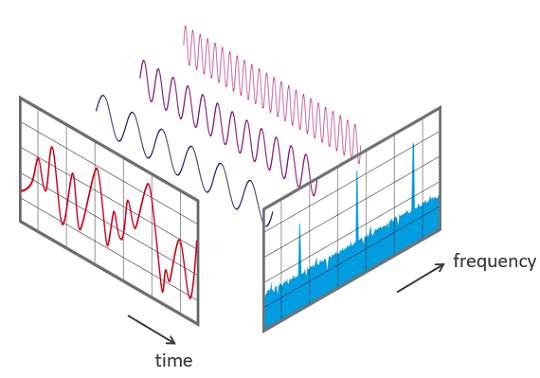
\includegraphics[width=0.6\textwidth]{k4.2/fourier.png}
    \caption{Anschauliche Darstellung der Fourier-Transformation (Quelle: www.nti-audio.com)}
    \label{k4.2.fourier.img}
\end{figure}

Ein anschauliches Beispiel ist die Spektralanalyse von Schallwellen. Die Daten (in der \cref{k4.2.fourier.img} links), die man beispielsweise mit einem Mikrofon aufnimmt, bestehen aus Schallwellen unterschiedlicher Wellenlängen. Mithilfe der Fourier-Transformation wird das Signal auf Schwingungen mit verschiedenen Wellenl\"angen aufgeteilt (in der \cref{k4.2.fourier.img} rechts), wodurch man das Frequenzspektrum erhält.

Je nachdem, welche Art von Rohdaten man erhält und welche Ausgabe erwünscht ist, nimmt die Fourier-Transformation eine leicht andere Form an.

Die kontinuierliche Fourier-Transformation (FT) benötigt als Eingabe eine Funktion, über die mit
\begin{displaymath}
\mathcal{F}(x)(s)=\int_{-\infty}^{\infty}e^{-ist}x(t)\ dt
\end{displaymath}
integriert wird. Diese Transformation lässt sich nur auf kontinuierliche Funktionen anwenden und gibt eine kontinuierliche Funktion aus.

Die diskrete Fourier-Transformation (DFT) kommt mit diskreten Werten aus und ist daher am Besten für digitale Signalverarbeitung geeignet, da die Eingabesignale meinstens aus einzelnen Datenpunkten und nicht aus kontinuierlichen Funktionen bestehen. Die Formel dazu ist entsprechend kein Integral, sondern eine Summe aller gegebenen Datenpunkte: 
\begin{displaymath}
\hat a_k = \sum\limits_{j=0}^{N-1}e^{-2\pi i\cdot\frac{jk}{N}}\cdot a_j.
\end{displaymath}
Die DFT ist mit einer quadratischen Laufzeit allerdings vergleichsweise rechenintensiv. Stattdessen wird in der Signalverarbeitung meist die Fast Fourier Transformation (FFT) verwendet, welche mit Hilfe des \emph{Divide and Conquer} (Teile-und-Herrsche) Prinzips in der Lage ist, die Rechenzeit drastisch zu reduzieren.

Manche Probleme, welche im Wertebereich, den eigentlichen Signalen, nur durch viele komplizierte Operationen l\"osbar sind, k\"onnen im Bildbereich, dem durch die Fourier-Analyse berechneten Frequenzspektrum, mit wenigen einfachen Operationen gel\"ost werden. Dazu wendet man die Fourier-Analyse auf die Daten an, führt die notwendigen Operationen im Bildbereich aus und transformiert die Lösung zurück in den Wertebereich. Möchte man beispielsweise eine Tonaufnahme von Störsignalen bereinigen, wendet man die FFT an, löscht die unerwünschten Frequenzen im Bildbereich und übersetzt das Ergebnis zurück in Musik oder Sprache. Diese Aufgabe w\"are im Wertebereich erheblich rechenintensiver gewesen, da an einer Tonaufnahme über der Zeit nicht direkt das Störsignal ablesbar ist.

Das \enquote{Rückübersetzen} der Signale erfolgt mit der inversen (kontinuierlichen oder diskreten) Fourier-Transformation (IFT). Diese erzeugt die Funktion oder eine Menge von Datenpunkten, welche aus einem gegebenen Spektrum entsteht. Dazu werden dieselben Operationen wie bei der Berechnung des Spektrums lediglich mit anderen Faktoren angewandt.




\section{Radioastronomie}
\sectionauthor{Constantin Burmeister, (Ole Fleck)}

Radioastronomie dient der Beobachtung von astrophysikalischen Prozessen, die Radiowellen, also Wellen langer Wellenlänge, aussenden. Um hohe Auflösungen zu erreichen, werden Radiointerferometer verwendet, welche Signale mehrerer Antennen so zusammenfügen, als würde es sich um eine Antenne handeln.

Allgemein ist der minimal auflösbare Bildwinkel $\delta\theta$ eines Teleskops abhängig von der Wellenlänge $\lambda$, des beobachteten Lichts, und dem Spiegeldurchmesser $D$ des Teleskops mit \begin{eqnarray}
\delta\theta\approx1.22\frac{\lambda}{D}
\end{eqnarray}
Da die Radioastronomie große Wellenlängen verwendet, sind hier auch bei Teleskopen mit großen Spiegeldurchmessern von über $100\text{m}$ nur geringe Auflösungen möglich.

\subsection{Radiointerferometrie}
\begin{figure}[htb]
\centering
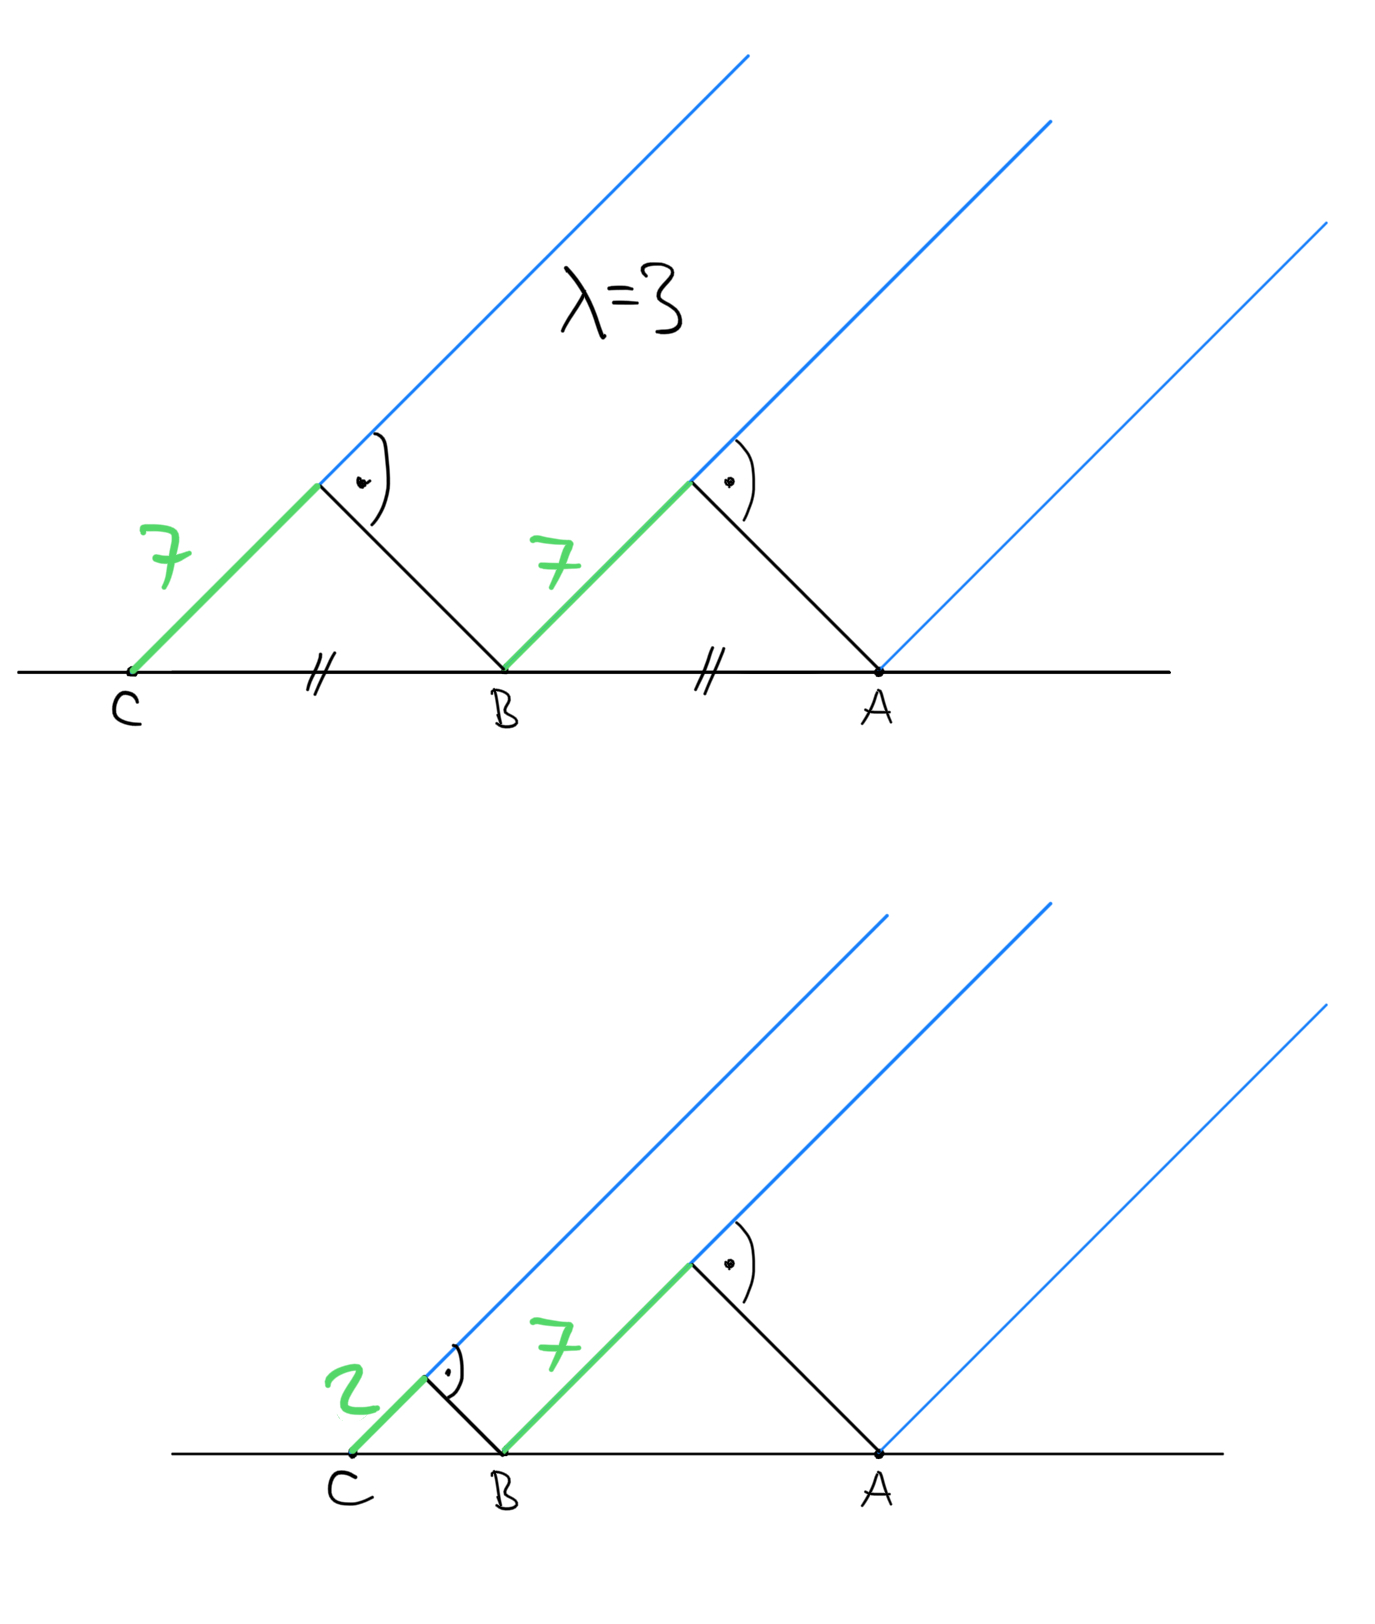
\includegraphics[width=.4\textwidth]{k4.2/baselineunterschied.png}
\caption{Gangdifferenzen von Radiowellen bei Antennenarrays}
\label{bild-baselineunterschied}
\end{figure}

Radiointerferometrie ist ein Verfahren zur Überlagerung von Radiowellen, welche von mehreren Antennen aufgezeichnet wurden, um eine höhere Auflösung zu erzielen als es mit einer einzelnen Antenne möglich wäre.

Das hieraus resultierende Signal ist vergleichbar mit dem Signal, welches von einer Antenne mit dem Spiegeldurchmesser entsprechend des Antennenabstandes erzeugt worden wäre.

Ein Interferometer kann nur die Laufzeitdifferenz zwischen Wellen bestimmen, da die einzelnen Wellenberge nicht unterschieden werden können. So können, wie im Beispiel  \cref{bild-baselineunterschied}, bei gleichen Abständen zwischen den Teleskopen A,B und C nicht zwischen den Gangdifferenzen modulo der Wellenlänge, welche im Beispiel $\lambda = 3$ beträgt, unterschieden werden. In diesem Beispiel ist aus den Messwerten nicht ersichtlich, ob es sich tatsächlich um $2\cdot \lambda +1 = 7$ Gangunterschied handelt, sondern jedes $n\in \mathbb{N}$ in $n\cdot\lambda+1$ ist möglich. Die Differenz könnte also immer auch um vielfache von 3 Längeneinheiten verschieden sein. Werden Antennen mit unterschiedlichen Abständen verwendet, sinkt die Anzahl der Kombinationen der Gangunterschiede, für welche sich eine solche Gleichung lösen lässt, wie im Beispiel, wo die Ergebnisse der Gleichung für das untere Bild kongruent zu 3 $\mathrm{mod}\,2$ sein müssen. Daher werden bei Antennengruppen möglichst viele unterschiedliche Abstände verwendet.

Für die Messung des Radiosignals gilt:
\begin{eqnarray}
d_{uv\lambda} =\int\int I(l,m)e^{-2\pi i \frac{1}{\lambda}(lu-mv)dldm}
\end{eqnarray}
Hier bezeichnet $l$ die Nord-Süd-Achse und $m$ die Ost-West-Achse, $\lambda$ bezeichnet die Beobachtungswellenlänge, und $u$ und $v$ ist der Verbindungsvektor zwischen zwei Antennen. Zusätzlich bezeichnet $n_{uv\lambda}$ ein additives Rauschen. Diese Messgleichung hat große Ähnlichkeit zur Fourier-Transformation (siehe \cref{k4.2.fourier}) und kann als nicht-äquidistante Fourier-Transformation interpretiert werden.

Dieses Verfahren wurde beispielsweise auch beim \emph{Event Horizon Telescope} verwendet. Das \emph{Event Horizon Telescope} besteht aus einer Verschaltung von elf Teleskopen, wobei deren Abstand bis zu $10000\,\text{km}$ beträgt. Mit diesem Teleskop wurde das erste Mal der Schatten eines Schwarzen Lochs beobachtet.

Radiointerferometrie ist also ein essenzieller Bestandteil der Astronomie. Das Verfahren ermöglicht die Ursprungsbestimmung eines Radiosignals von astrophysikalischen Prozessen bei hoher Auflösung.



\section{Tomographie}\label{k4.2.comptomo.ct}
\subsection{Einleitung}
\sectionauthor{Aaron Gschwendt (Finja Hoffmann)}

Die Tomographie ist ein bildgebendes Verfahren, in dem ein Objekt schichtweise untersucht wird. Um diese Schichten zu vermessen, beobachtet man Strahlen, die das Objekt schneiden und auf einer Ebene liegen. Die Menge an Licht, die auf der Strecke absorbiet wurde, entspricht dem Linienintegral:

$$d=\int_{\Gamma}{}s(p)dp(\gamma)$$

$s$ ist eine unbekannte Funktion die jedem Punkt im Raum eine optische Dichte zuordnet. $d$ ist das Linienintegral von $s(p)$ entlang dem Pfad $\gamma$. $d$ entspricht der Menge an Licht, die zwischen dem Sender und dem Empfänger absorbiert wird und wird experimentell bestimmt.

Gesucht ist die Funktion $s$, diese lässt sich jedoch nicht analytisch bestimmen. Kennt man aber $d$ von genug Linien in $s$, kann man mithilfe des Satzes von Bayes mit hoher Auflösung und Sicherheit $s$ bestimmen.

\subsection{Radioastronomie}

In der Astronomie wird die Tomographie z.B. verwendet, um die Form von kosmischen Wolken zu ermitteln. Dafür werden Sterne, deren absolute Helligkeit und Distanz bekannt ist beobachtet. Man vergleicht ihre scheinbare Helligkeit mit der zu erwartende Helligkeit und ermittelt so $d$ für alle Strecken zwischen der Erde und den beobachteten Sternen. $d$ entspricht in dem Fall die Menge an Staub zwischen dem Stern und der Erde. Aus vielen (Distanz, Helligkeit)-Paaren kann man $s$ lernen und Aussagen über die dichte-Verteilung und Form der Wolke treffen.

\subsection{Computertomografie}

Häufig verwendet wird die Tomographie auch in der Medizin, bekannt als Computertomographie(CT).

Bei herkömmlichen Röntgenuntersuchungen werden Röntgenstrahlung durch das abzubildende Objekt auf einen Röntgenfilm oder einer Sensorplatte geleitet. Das 3d-Objekt wird dabei auf eine 2d-Fläche projeziert. Der Nachteil dieser Methode ist, dass sich Teile vom Objekt überlagern können und nicht erkannt werden kann, ob es sich um ein Objekt mit hoher Absorption oder mehrer Objekte mit geringer Absorption handelt.

Beim CT drehen sich im $180^\circ$ Winkel eine Röntgenröhre und Detektor um den Patienten und nehmen dabei in kleinen Abständen Messpunkte auf. Dies wird für mehrere Schichten entlang des zu untersuchenden Körperteils ausgeführt. Der Röntgenstrahl und Detektor ist breit genug, dass bei jedem Messpunkt die ganze Breite des Körperteils in einem Streifen ergriffen wird.

\begin{wrapfigure}{r}{0.4\linewidth}
 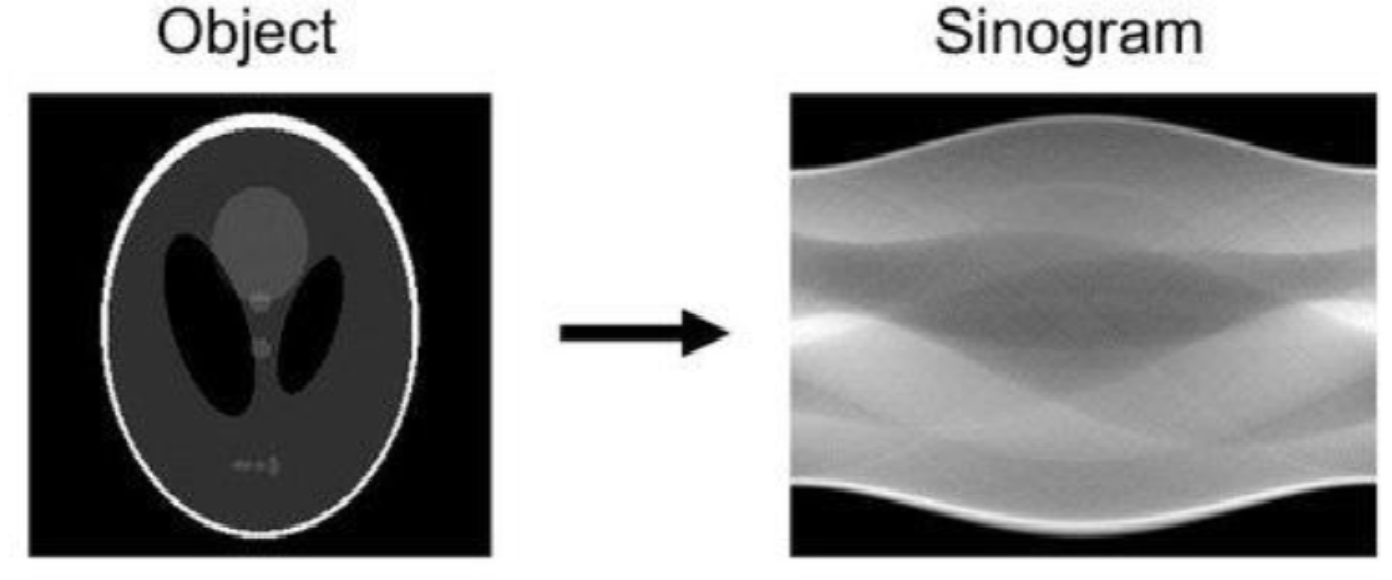
\includegraphics[width=0.4\textwidth]{k4.2/backprojektion.png}
 \caption{Sinogram}
 \label{k4.2.tomo.ct.bp}
\end{wrapfigure}

Daraus entsteht für jede Schicht ein Sinogram \cref{k4.2.tomo.ct.bp} bei der eine Achse (hier Y-Achse) das Absorptionsprofil und die andere (hier X-Achse) dem Winkel entspricht. Jede Stelle im Objekt bildet eine Sinuskurve; ihr Abstand vom Mittelpunkt entspricht der Amplitude und ihr Winkel im vergleich zum Startpunkt der Phasenverschiebung der Sinuskurve. Mit dem bayeschen Verfahren  kann man ein Bild von der Schicht mit hoher Genauigkeit rekonstruieren. Macht man dies für jede Schicht erhält man ein 3d-Rendering des Objekts.


\subsection{CT in 3D}
\sectionauthor{Finja Hoffmann, Chuyang Wang}

Im Rahmen der Projektarbeit soll aus den gemessenen Daten $d$ die Funktion des Signals $s(p)$ (\emph{quantity of interest}) in Abhängigkeit von einem 3D-Punkt $p \in \mathbb{R}^3$ rekonstruiert werden, welche die Dichte eines Objekts in einem diskreten 3-dimensionalen Raum beschreibt. Generell lässt sich der Datenvektor $d \in \mathbb{R}^N$ wie folgt berechnen:

\begin{equation}
  \begin{aligned}
    d = Rs + n,
  \end{aligned}
\end{equation}

wobei jeweils $R \in \mathbb{R}^{N \times M}$ das \emph{Response}, $s \in \mathbb{R}^M$ die Signale und $n \in \mathbb{R}^N$ das Rauschen beschreiben. Jede Komponente von $d$ entspricht einem Linienintegral aus \cref{k4.2.tomo.einl.linig}.
% TODO: ref to Wiener Filter

\subsection{Line-Of-Sight Response}
\sectionauthor{Finja Hoffmann, Chuyang Wang}

Angenommen, die Start- und Endpunkte der Messungen seien bereits gegeben und bilden jeweils die Strecken. Aus diesen Daten kann man die Matrix $R$ konstruieren. Anders gesagt repräsentiert $R$ die Start- und Endpunkten. Da die Signale in Form von diskreten Datenwürfel angegeben sind, ist $R$ also eine Gewichtung der gegebenen Signale. Als Gewichtung eines Datenwürfels gilt der euklidischen Abstand zwischen den beiden Schnittpunkten der Strecke mit den Seiten des Würfels. \textcite{k4.2.siddon} hat dafür einen effizienten Algorithmus geliefert, dessen Ansatz hier umgesetzt wird.


\subsection{Algorithmus von Siddon}

Siddons Ansatz nach könnte man die Schnittpunkte einer Sichtlinie mit den x-, y- und z-Achsenebenen jeweils einzeln bestimmen und in sortierte Listen $A$, $B$ und $C$ speichern. Sei jeweils

\begin{equation}
  P_{start} = \begin{pmatrix}x_{start} \\ y_{start} \\ z_{start}\end{pmatrix}
\end{equation}

\begin{equation}
  P_{end} = \begin{pmatrix}x_{end} \\ y_{end} \\ z_{end}\end{pmatrix}
\end{equation}

Betrachtet man zunächst die x-Achsenebene. Ohne Beschränkung der Allgemeinheit sei $x_{start} < x_{end}$. Man rundet die x-Koordinate des Startpunktes in die Richtung der Strecke auf und berechnet die Differenz $x^{\ast}$. Um die y- und z-Koordinaten dieses ersten Schnittpunkts herauszufinden, muss man noch die Steigungen gegenüber dieser beiden Achsen $m_{yx} = \frac{y_{end} - y_{start}}{x_{start} - x_{end}}$ und $m_{zx} = \frac{z_{end} - z_{start}}{x_{start} - x_{end}}$ berechnen. Somit erhält man den ersten Schnittpunkt

\begin{equation}
  S_{x,0} = \begin{pmatrix}
    x_{start} + x^{\ast} \\
    y_{start} + x^{\ast} \cdot m_{yx} \\
    z_{start} + x^{\ast} \cdot m_{zx} \\
  \end{pmatrix}
\end{equation}

Die weiteren Schnittpunkte $S_{x,i}$ kann man rekursiv konstruieren, indem man jeweils eine Einheit in die x-Richtung geht und die Änderungsrate gegenüber der y- und z-Achsen jeweils aufaddiert, also nämlich

\begin{equation}
  S_{x,i} = S_{x,i-1} + \begin{pmatrix}
    1 \\
    1 \cdot m_{yx} \\
    1 \cdot m_{zx} \\
  \end{pmatrix}
\end{equation}

 Die Liste $A$ besteht aus allen Schnittpunkten $[S_{x,0}, S_{x,1}, ..., S_{x,n}]$. Die Listen $B$ und $C$ berechnet man analog.

Anschließend muss man die drei Listen in eine einzelne sortierte Liste $\mathbf{S}$ zusammenführen. Diese geschieht, indem man alle Schnittpunkte aus $A$, $B$ und $C$ nach den x-Koordinaten aufsteigend sortiert. Sollte $x_{start} = x_{end}$ sein, dann nutzt man die y- oder z-Achse als den Sortierschlüssel.

Hat man alle sortierten Schnittpunkte, so kann man auch die Gewichtungen, i.e. die Abstände zwischen den jeweiligen Punkten, einfach berechnen. Jede dieser Gewichtungen wird einem Datenwürfel zugeordnet, durch den diese Teilstrecke durchdringt. Für diese Sichtlinie kann dann ein Zeilenvektor $r_i$ erstellt werden, welcher diese Zuordnung von Gewichtungen speichert. Man beobachte, dass jede Sichtlinie nur wenige Datenwürfel im 3D-Raum durchgeht. Also sind die meisten Gewichtungen für diese Sichtlinie null.

Daraus entsteht für jede Schicht ein Sinogram (Abbildung 1.1), bei dem eine Achse (hier Y-Achse) das Absorptionsprofil und die andere (hier X-Achse) dem Winkel entspricht. Jede Stelle im Objekt bildet eine Sinuskurve; Ihr Abstand zum Mittelpunkt entspricht der Amplitude und ihr Winkel die Phasenverschiebung. Mithilfe vom Satz von Bayes kann man ein Bild von der Schicht rekonstruieren. Macht man dies für jede Schicht erhält man ein 3d-Rendering.


\subsection{Walnuss -Messdaten}\label{k4.2.ch.walnussct}
\sectionauthor{Leo Bergmann, Cedric Balzer}

\begin{figure}
    \centering
    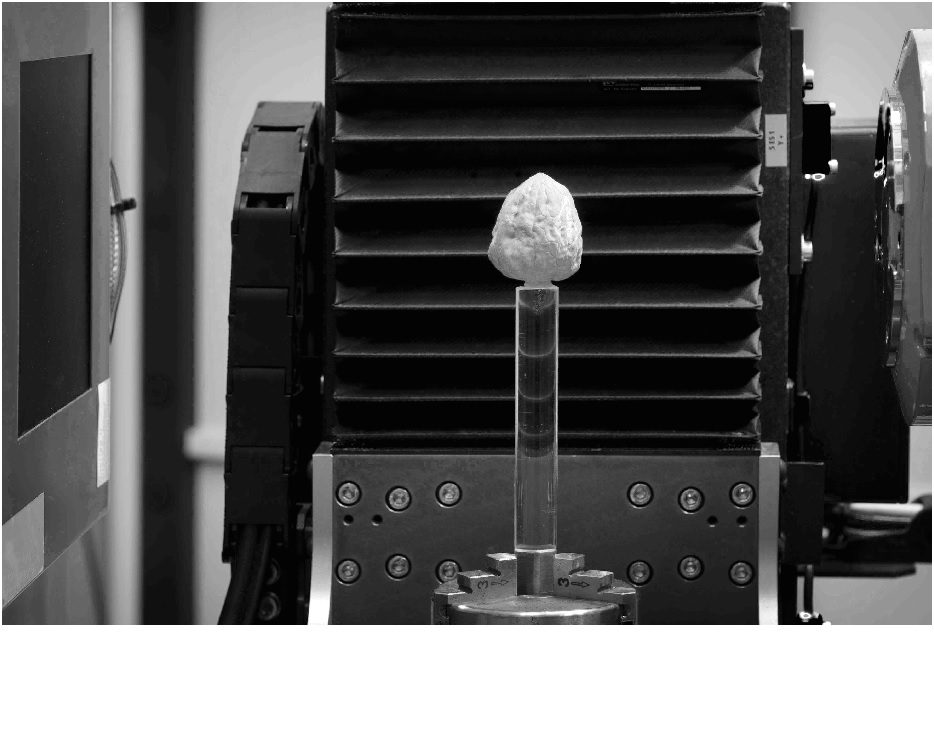
\includegraphics[width=0.7\textwidth]{k4.2/ctabbild.png}
    \caption{Versuchsaufbau, welcher für das Generieren der Daten verwendet wurde. Die Detektorfläche ist auf der linken Seite die Röntgenquelle auf der rechten Seite. Die Walnuss ist mit einer computergesteuerten rotierbaren Plattform verbunden.}
    \label{k4.2.fig.ctAbbild}
\end{figure}
\begin{figure}
    \centering
    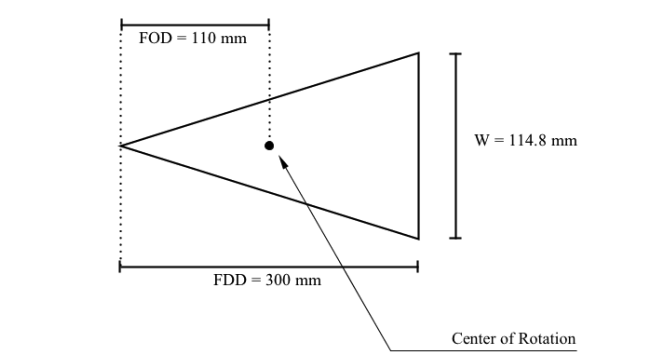
\includegraphics[width=0.9\textwidth]{k4.2/geometry.png}
    \caption{Aufbau des Versuchs mit geometrischen Daten.\\
    FOD - Focus-to-object distance\\
    FDD - Focus-to-detector distance\\
    W - Width of the detector
    }
    \label{k4.2.fig.Geo}
\end{figure}

Das Ziel des Projekts ist es, einen Computertomographie-Scan (siehe \cref{k4.2.comptomo.ct}) einer Walnuss als Bild darzustellen. Durch die harte Schale und den weichen Kern stellt die Walnuss eine Herausforderung für den CT-Scan dar.
Wir beziehen öffentlich zugängliche Daten von  \href{https://zenodo.org/record/1254206#.Ys6OHnZBw7c}{zenodo.org}, die eine Schichtaufnahme einer Walnuss als Sinogram in unterschiedlichen Auflösungen in \verb|.mat|-Dateien beinhalten. 
Es wurden 120 Projektionen der Strahlung auf einem Schirm gemessen und mit einer heruntergerechneten Pixelzahl in einer Matrix m gespeichert. Getestet haben wir Dateien mit 82 und 328 Pixel je Projektion. In dem Versuch wurde eine Walnuss zwischen eine punktförmige Strahlungsquelle und einen flachen Schirm positioniert (\cref{k4.2.fig.ctAbbild}). Nach jeder Messung wurde die Nuss um 3° gegen den Uhrzeigersinn gedreht. Damit das Sinogram in ein CT-Bild projiziert werden kann sind alle Start- und Endpunkte der Line of Sight notwendig. Diese werden ermittelt, indem der Standort der Quelle und die Position der einzelnen Pixel des Screens ermittelt wird. 

\begin{figure}
    \centering
    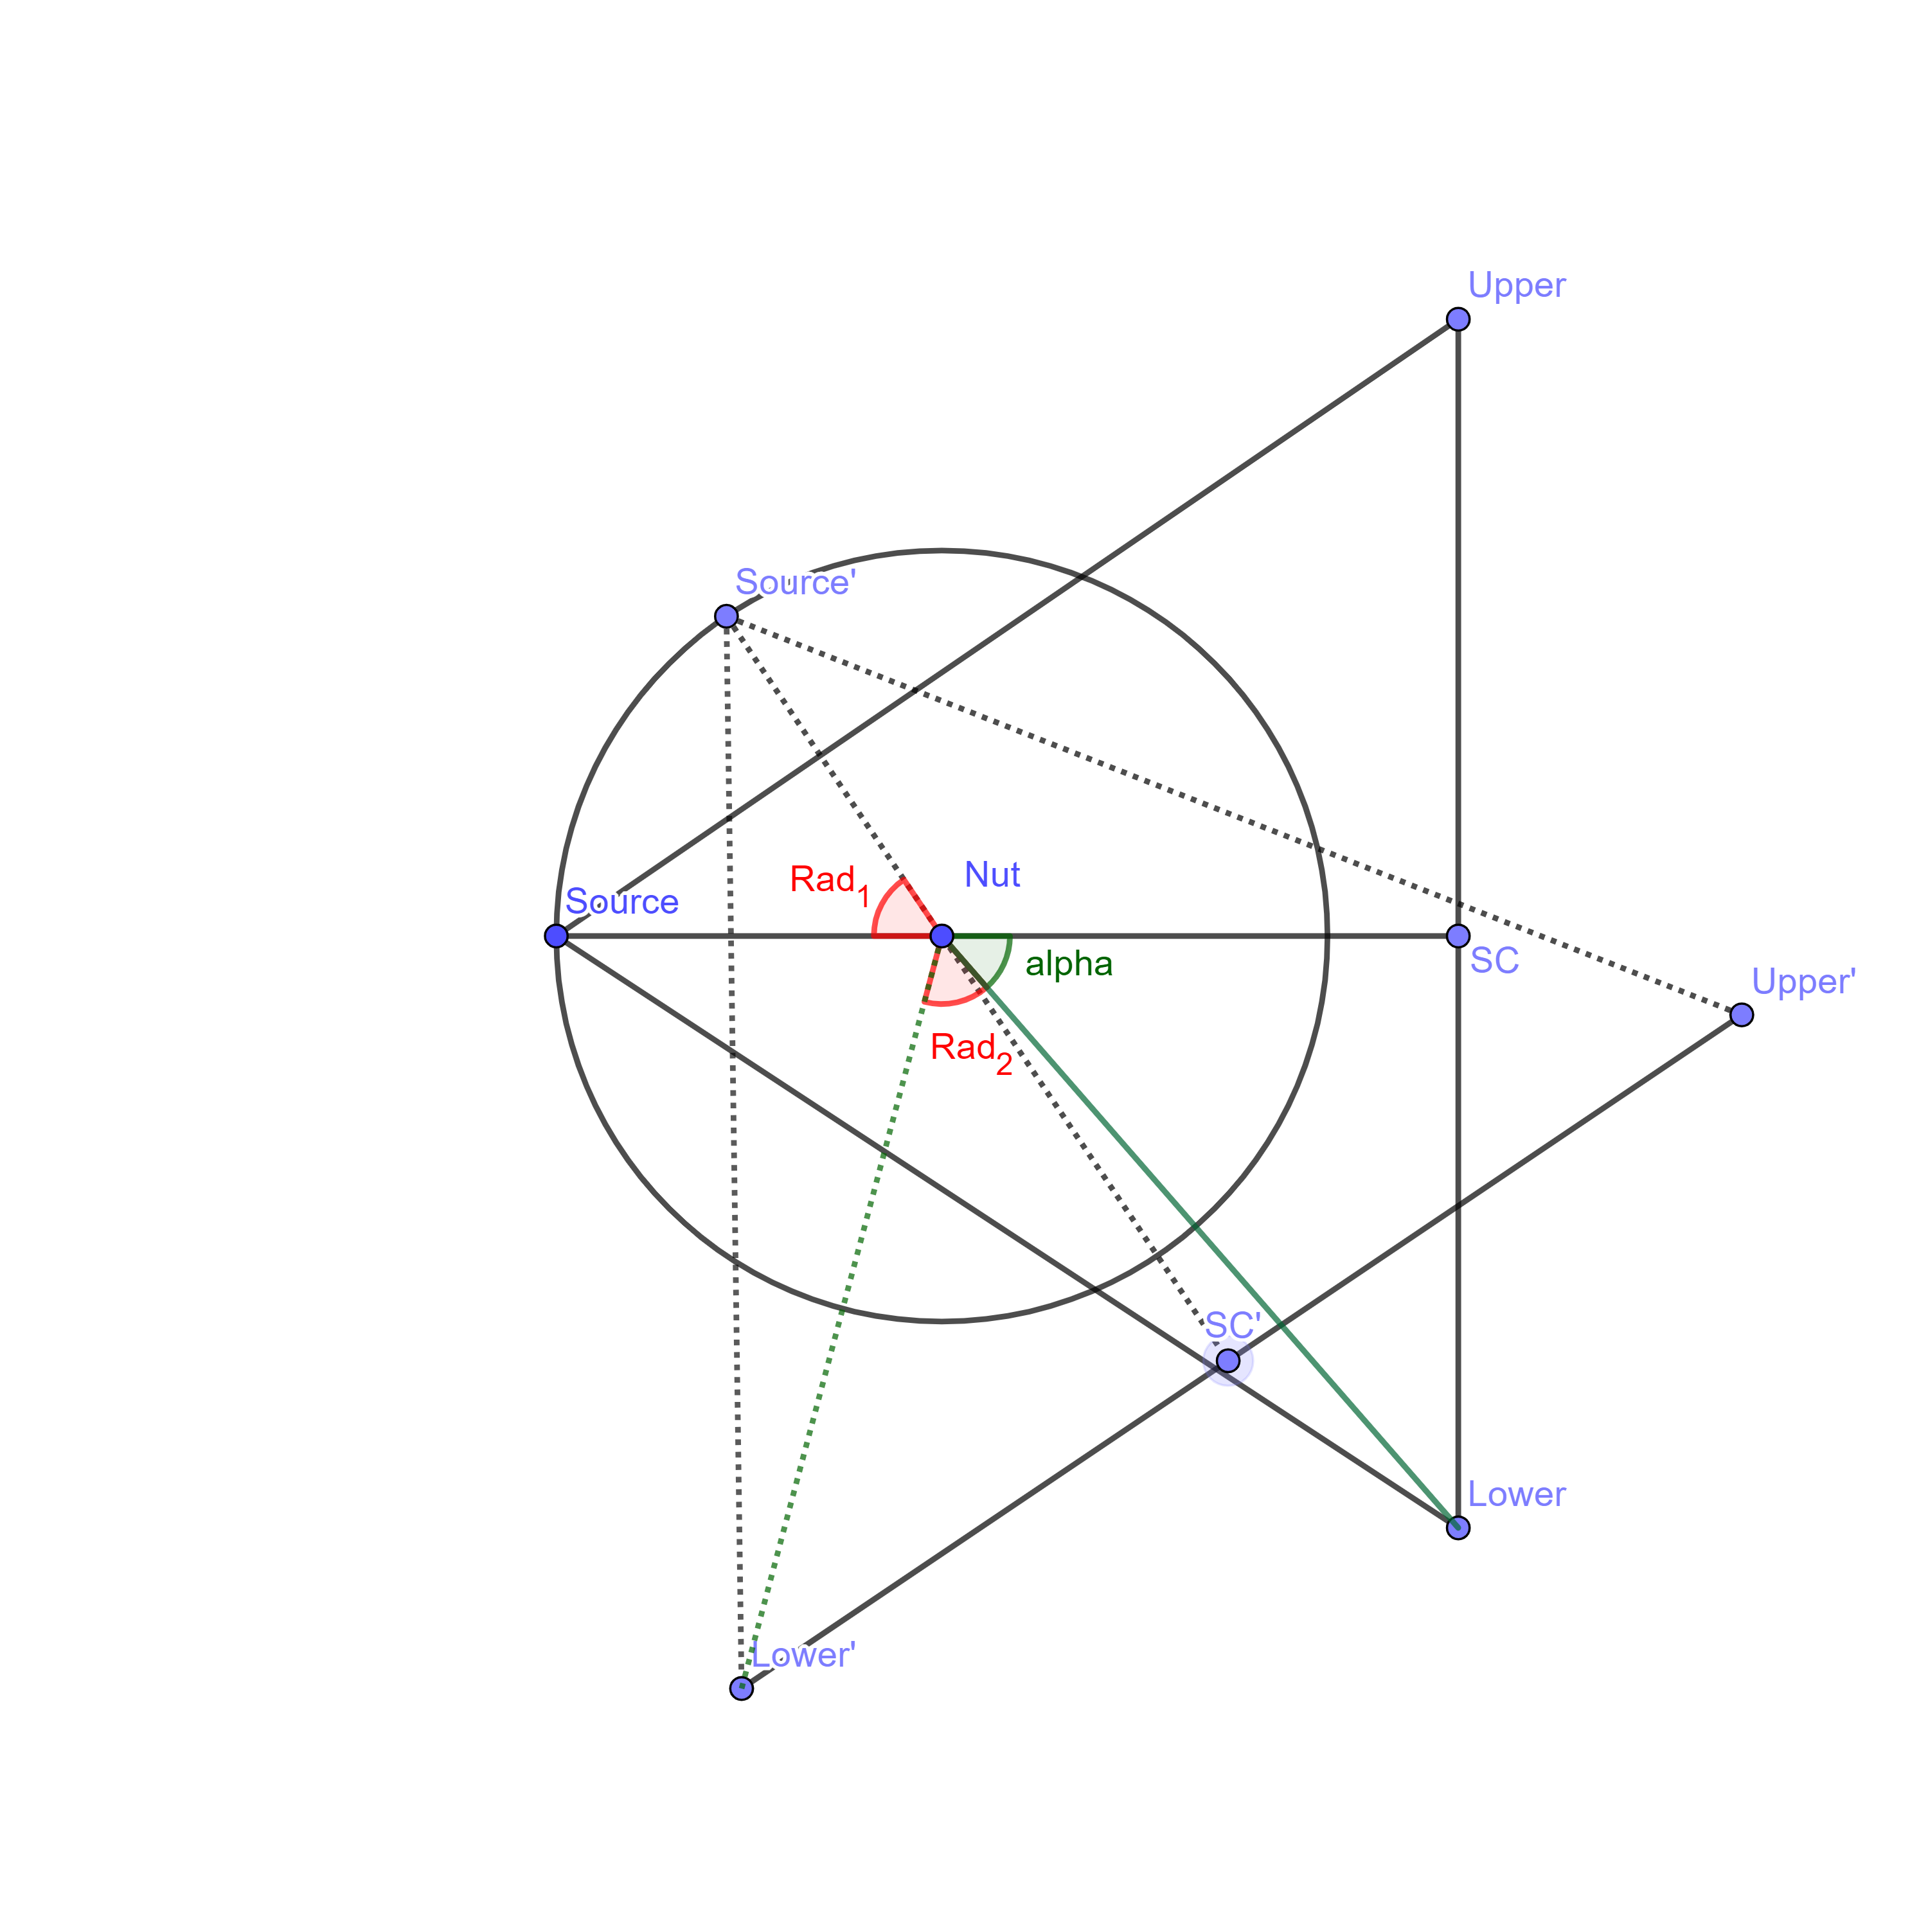
\includegraphics[width=0.9\textwidth]{k4.2/versuchsaufbau-skizze.png}
    \caption{Skizze des Versuchsaufbau}
    \label{k4.2.fig.skizze}
\end{figure}
Anstelle einer Drehung der Nuss gegen den Uhrzeigersinn rechnen wir, äquivalent dazu, mit einer kreisförmigen Rotation des Detektors (Screen) und der Strahlungsquelle (Source) um die Walnuss (Nut). Es bieten sich durch gegebene Winkel und Radii Polarkoordinaten an, um die Position der Quelle und des Detektors relativ zu Walnuss zu bestimmen, jedoch müssen alle Punkte für die Weiterverarbeitung im kartesischen Koordinatensystem angegeben und deshalb direkt in diesem berechnet werden. Da die Winkel und Abstandsmaße in Bezug auf die Walnuss angegeben sind, wird diese als Koordinatenursprung definiert. Ausgehend davon wird die Quelle zunächst an die Stelle \verb+(-110|0)+ gelegt (siehe \cref{k4.2.fig.Geo}). Dadurch wird die Startposition des Detektors festgelegt, der durch seinen Anfang ($Upper$) an Stelle \verb+(190|57,4)+ und seinen Endpunkt ($Lower$) an Stelle \verb+(190|-57,4)+ bestimmt wird. 
Source' ist für jede Drehung der Nuss bzw. der Quelle und des Schirms um den Winkel Rad (im Bogenmaß) im Vergleich zur Startposition der Punkt an dem sich die Quelle nun befindet. Der Abstand zwischen Source' und Nut ist dabei immer 110mm. Der Versuchsaufbau kann somit als Einheitskreis mit Mittelpunkt Nut interpretiert werden, der um den Faktor 110mm gestreckt wurde. Dadurch ist im karthesischen Koordinatensystem die horizontale Koordinaten-Komponente von Source' gleich $cos(Rad) * 110mm$, die vertikale Komponente gleich $sin(Rad) * 110mm$.
Der Winkel $\sphericalangle Upper-Nut-Lower$ hat eine Größe von etwa 34°, somit hat der Winkel $alpha = \sphericalangle Lower-Nut-SC$ eine Größe von 17°. Der Abstand von Nut zu $Lower$ kann mithilfe des Satzes von Pythagoras berechnet werden:
\begin{align}
d = \sqrt{(300mm - 110mm)^2+(114,8mm/2)^2} = 198,48mm
\end{align}
Der Winkel $alpha$ addiert mit Rad ergibt zusammen mit der Länge $d$ die Koordinaten $alphas$ im Polarkoordinatensystem (Winkel werden im Bogenmaß verrechnet). Um $Upper'$ zu berechnen muss $alpha$ von Rad subtrahiert werden. Die entsprechenden karthesischen Koordinaten erhalten wir nun auf gleiche Weise bei Source'. Um die restlichen Pixel zu berechnen verwenden wir die Methode \verb+numpy.linspace()+. Wir setzen hier $Upper'$ als Startwert und $Lower'$ als Endwert ein und lassen uns die Menge der Anzahl an Pixeln auf dem Schirm ausgeben. 

Die erhaltenen Start und Endpunkte, in Kombination mit den im Datenset gelieferten Helligkeitswerten kann nun in ein vollständing rüchprojeziertes CT Schichtbild verwandelt werden.


\section{Wiener Filter}\label{k4.2.wiener.filter}
\sectionauthor{Constantin Burmeister, Clemens Ljungh, Natalie Teplitska}

Für unseren Kurs benötigen wir eine Möglichkeit, aus Rohdaten auf das zugrundeliegende physikalische Signal zurückzuschließen. Allerdings können Messungen nur mit einer endlichen Sicherheit erfolgen, was bildgebende Verfahren vor Probleme stellt. So lässt sich Rauschen sowie eine gewisse Ungenauigkeit in der Messung nicht vermeiden; zudem sind die Daten unvollständig. Um solche Probleme zu lösen, brauchen wir den Wiener Filter.
Dieses mathematische Verfahren basiert auf dem Bayes'schen Theorem
(\ref{k4.2.bayes})
, welches mathematisch beschreibt, wie Wissen optimal verändert werden muss, nachdem Daten erhoben wurden. Der Wiener Filter kann nur verwendet werden, wenn sowohl der Prior als auch die Likelihood normalverteilt sind.

Der Wiener Filter kann verwendet werden, wenn die zwei folgenden Annahmen erfüllt sind. Zum Einen setzt man voraus, dass a priori das untersuchte Signal Gauß-verteilt ist: $P(s) = \mathcal{G}(s,S)$. Zum Anderen ist das Rauschen normalverteilt mit $P(n) = \mathcal{G}(n,N)$ und additiv. Aus der Normalverteilung des Rauschens sowie unter Einbezug der Messgleichung ergibt sich auch eine Normalverteilung für die Likelihood. Der Messoperator $R$ muss linear sein. Insgesamt ergibt sich folgende Messgleichung:
\begin{eqnarray}
d = Rs + n
\end{eqnarray}
In der Formel beschreibt $d$ die Daten und $s$ die Quantity of Interest, also das ursprüngliche Signal. $R$ ist die Response, das heißt die Abbildung des Signals in den Datenraum. Die Wahrscheinlichkeit, die Daten $d$ für das Signal $s$ zu erhalten, ist eine Gauß-Verteilung.
\begin{eqnarray}
P(d|s) = \mathcal{G}(d-Rs,N)
\end{eqnarray}
Setzen wir $P(s)$ und $P(d|s)$ in Bayes ein \cref{k4.2.bayes} erhalten wir:
\begin{eqnarray}
P(s|d) = \mathcal{G}(s-m,D)
\end{eqnarray}
mit:
\begin{eqnarray}
D^{-1} = R^{\dagger} N^{-1}R + S^{-1}
\end{eqnarray}
und
\begin{eqnarray}
m = D R^{\dagger} N^{-1}d
\end{eqnarray}
Der Posterior $P(s|d)$ ist also auch eine Gauß-Verteilung und hat den Erwartungswert $m$. Der Wiener Filter ist insofern vorteilhaft, als dass er mit beliebig wenigen Daten fehlerfrei funktioniert, und ist daher eine wichtige Methode der IFT.


\section{Normalverteilung}
\sectionauthor{Patricia Hackl, Lara Müller}

Im Hinblick auf die Bayes'sche Wahrscheinlichkeitstheorie ist die Gauß'sche Normalverteilung (auch: Gauß'sche Glockenkurve) von Bedeutung.
Es lässt sich zeigen, dass die Summe von identisch verteilten und voneinander unabhängigen Zufallszahlen im Limes (Anzahl Wiederholungen $\rightarrow \infty$) zur Normalverteilung konvergiert.
Die einem Zufallsexperiment zugehörige Gauß'sche Normalverteilung ist vollständig definiert über ihren Erwartungswert $\bar{x}$ und die Varianz $\sigma^{2}$:
\[ \mathcal{G} (x - \bar{x}, \sigma^{2}) = \displaystyle\frac{1}{\sqrt{2 \pi \sigma^{2}}} \exp \left(- \displaystyle\frac{1}{2} \cdot (x - \bar{x}) \cdot (\sigma^{2})^{-1} \cdot (x - \bar{x}) \right) \]
Analog zur Summenregel gilt auch für das Integral über die Normalverteilung:
\begin{center} $\int_{- \infty}^{\infty} \mathcal{G} (x - \bar{x}, \sigma _x ^{2}) dx = 1$ \end{center}

\subsection{Erwartungswert}
Der Erwartungswert selbst ist definiert als die gewichtete Summe aus den Wahrscheinlichkeiten für die Zufallsvariable $x _i$ und bestimmt in spezifischen Fall der Normalverteilung, an welcher Stelle das Maximum auftritt (Verschiebung der Glockenkurve entlang der x-Achse). Dieser Wert muss nicht zwangsweise realisierbar sein. In der Formel entspricht $\chi$ dem Raum, auf dem $P(x)$ definiert ist:
\begin{center} $\mathbb{E} _{P(x)} [x] = \sum x _i P(x _i) = \int_{\chi} x P(x) dx$ \end{center}

\subsection{Varianz und Standardabweichung}
Genauer betrachtet stellt die Varianz die Streuung um den Erwartungswert dar und entspricht somit der Abweichung vom Mittelwert. Diese ist immer strikt positiv.
\begin{center} $\mathrm{Var} _{P(x)} [x] = \mathbb{E} _{P(x)} [x^{2}] - (\mathbb{E} _{P(x)} [x])^{2} = \int_ {\chi} (x - \mathbb{E} _{P(x)} [x])^{2} P(x) dx \geq 0$ \end{center}
Für die Standardabweichung $\sigma$, die das Maß der Streubreite beschreibt, ergibt sich folgende Formel, wodurch eine direkte Abhängigkeit von der Varianz deutlich wird:
\begin{center} $\sigma _{P(x)} [x] = \sqrt{\mathrm{Var} _{P(x)} [x]}$ \end{center}

Mithilfe der Gauß'schen Glockenkurve lassen sich nun vielfältige Zufallsexperimente beschreiben und entsprechende Wahrscheinlichkeitsverteilungen konstruieren. In Bezug auf den Wiener Filter wird die Normalverteilung nicht nur als Prior, sondern auch als Likelihood benötigt, um Datenlücken zu füllen, die aufgrund des Abstands der Antennen des Radioteleskops auftreten. Zudem ist das Rauschen, also die Ungenauigkeit in den Messdaten, normalverteilt und kann so aus den Daten extrahiert werden.



\section{Inferenz - Lernen aus Daten}
\sectionauthor{Natalie Teplitska, Clemens Ljungh, Constantin Burmeister}
Mit dem Wiener Filter \cref{k4.2.wiener.filter} besitzen wir ein Werkzeug, unser Wissen über die Welt aufgrund von Daten beständig anzupassen. Allerdings gilt der Wiener Filter nur für den Spezialfall, dass $d=Rs+n, P(s)=\mathcal{G}(s,S), P(n) = \mathcal{G}(n,N)$ gilt.

Unser Ziel ist es nun, aus den Daten das ursprüngliche Signal, welches diese Daten verursachte, zu rekonstruieren. Dazu müssen wir - bildlich gesprochen - die Formel $d=Rs+n$ invertieren und so die quantity of interest $s$ bestimmen. Aus diesem Grund wird die Fragestellung als inverses Problem bezeichnet.

Betrachten wir es aus der Bayes'schen Perspektive. Der Posterior ist zwar durch Messgleichung, $P(s)$, $P(n)$ und $R$ vollständig definiert, doch seine Berechnung ist insbesondere bei großen Datenmengen, wenn der Posterior nicht analytisch lösbar ist, viel zu rechenintensiv und somit teuer. Zur Bewältigung dieser Herausforderung existieren zwei Lösungsansätze.

Das Verfahren Markov-Chain-Monte-Carlo basiert darauf, dass aus $P(s|d)$ lediglich Stichproben gezogen werden und dadurch eine optimale Lösung gefunden wird. Leider ist auch diese Methode noch zu rechenintensiv, weswegen wir sie nicht nutzen.

Eine weitere Möglichkeit besteht darin, den Posterior mit einem variativen Ansatz anzunähern. Dieser benötigt ein Maß für die Quantifizierung des Approximationsfehlers, welches mit der sogenannten Kullback-Leibler-Divergenz (KL-Divergenz) wie folgt definiert ist:
\begin{eqnarray}
\text{KL}(P,P_a) = \int P(s|d) ln \frac{P(s|d)}{P_a(s|d)}ds
\end{eqnarray}
Das Minimieren von $\text{KL}(P, Pa)$ liefert die optimale Approximation an den Posterior.

Die KL-Divergenz hat einige nennenswerte Eigenschaften. Dazu gehört unter anderem die Lokalität, die dazu führt, dass nur Stellen in die Fehlerberechnung einfließen, über welche die erste Verteilung $P$ eine Aussage trifft. Außerdem folgt die KL-Divergenz dem Konzept der Gescheitheit, welches besagt: \enquote{Wann immer möglich, wähle die zweite Verteilung $P_a$ so, dass diese mit der ersten übereinstimmt.} Zuletzt ist zu erwähnen, dass die KL-Divergenz invariant unter Koordinatentransformationen ist und sich daher nicht verändert, wenn die Koordinatenachsen transformiert werden.

Die KL-Divergenz wendet man beim Verfahren der variativen Inferenz an. Dabei minimiert man jedoch nicht $\text{KL}(P, P_a)$, sondern $\text{KL}(P_a, P)$, da diese Optimierung weniger rechenintensiv ist.

\section{Radiointerferometrie-Response und Event-Horizon-Telescope-Daten}
\sectionauthor{Alexander Gitnik, Jonas Fiedler, Lara Müller, Patricia Hackl}

Zur Rekonstruktion eines Bildes des Schwarzen Lochs M87* muss basierend auf den Daten des Event-Horizon-Telescopes zunächst eine Response-Funktion implementiert werden, um die Informationen vom Signal- in den Datenraum zu transferieren $s \mapsto d$. Mit der entsprechenden Implementierung wird sich der nachfolgende Abschnitt befassen.

Es werden Daten in Form von acht csv-Dateien verwendet, die im April 2017 aufgenommen wurden. Diese stammen von mehreren Messreihen und wurden zur weiteren Verarbeitung in Form von csv-Dateien gespeichert.
Um mit den Messwerten in Python arbeiten zu können, werden die csv-Dateien in NumPy-Arrays konvertiert. Durch das NumPy-Array werden die Daten aus den csv-Dateien auf einem zweidimensionalen Gitter abgebildet.

Zunächst müssen die Frequenzen der Radiowellen ausgelesen werden. Diese elektromagnetischen Wellen werden in unmittelbarer Nähe des Schwarzen Lochs ausgesandt. Es wurden die beiden Frequenzen $f_1 = 227,0707$ GHz und $f_2 = 229,0707$ GHz betrachtet. Darüber hinaus werden auch die Verbindungsvektoren zwischen den Antennen $uvw$ ausgelesen.

Um aus den Messwerten ein Bild erstellen zu können, wird die Anzahl der Pixel sowohl in x-, als auch in y-Richtung auf zunächst $100$ festgelegt, wobei dieser Wert variabel ist. Die Größe der Pixel ergibt sich für $\delta \theta$:
\[ \delta \theta = 1.22 \cdot \displaystyle\frac{\lambda}{D} = 1.22 \cdot \displaystyle\frac{c}{f \cdot D} \]

Da es sich bei dem Event Horizon Telescope um einen Zusammenschluss von Antennen auf der ganzen Welt handelt, ergibt sich ein Durchmesser von $D_{EHT} \approx D_{Erde} \approx 10.000km$. Desweiteren beschreibt $\lambda$ die Wellenlänge der Radiowellen und $c$ deren Ausbreitungsgeschwindigkeit, die der Lichtgeschwindigkeit entspricht. In die Formel eingesetzt erhält man:

\begin{equation}
  \delta \theta = 1.22 \cdot \displaystyle\frac{3 \cdot 10^{8} \displaystyle\frac{\text{m}}{\text{s}}} {229.0707 \text{GHz} \cdot 10.000 \text{km}} = (1,598 \cdot 10^{-10}) \mu \text{as} 
\end{equation}

Damit ein erstes Bild des Schwarzen Lochs generiert werden kann, ist es notwendig, die Daten $d$ mittels folgender Formel zu beschreiben. Die Werte für $I_{Amplitude}$ und $I_{Phase}$ sind in den csv-Dateien gegeben:
\[ d = I_{Amplitude} \cdot e^{i \cdot I_{Phase}} \]

Aufgrund unvollständiger Informationen, die durch die Distanz der Antennen des Event-Horizon-Telescopes entstehen, muss zur Bilderstellung Bayes'sche Statistik angewandt werden.Im Gegensatz zu NumPy stellt NIFTy entsprechende Funktionen bereit, die dies ermöglichen. Um vom Signalraum $I$ (Signal des betrachteten Objekts) in den Datenraum $d$ (empfangene Daten) zu gelangen, nutzt man in NIFTy die Funktion \verb|dirty2vis| aus der Python-Bibliothek \verb|ducc0|. Die adjungierte Abbildung \verb|vis2dirty| ermöglicht es, aus dem bekannten Datenraum auf den Signalraum zu schließen.\\
Um diese Funktionen in NIFTy wiederholt anwenden zu können, werden sie in eine Klasse verpackt. Es handelt sich dabei um eine Klasse, die von \verb|ift.LinearOperator| - einem NIFTy-Operator - erbt. Dazu müssen unter Anderem \verb|domain| und \verb|target| initialisiert werden. Der Signalraum wird über \verb|domain| beschrieben, der Datenraum über \verb|target|. In der Klasse werden die Funktionen \verb|dirty2vis| und \verb|vis2dirty| durch die Methoden \verb|TIMES| und \verb|ADJOINT_TIMES| ersetzt.



\section{Kalibrierung der Radiointerferometriedaten}
\sectionauthor{Benjamin Knöbel del Olmo, Ole Fleck, Aaron Gschwendt, Mara Germann}
Die Aufgabe dieses Projektteils war es, Daten, die Teil A (Ref!) simuliert, zu korrigieren. Im Gegensatz zu Beobachtungen durch einzelne Antennenarrays wurde das Schwarze Loch M87 durch das Event Horizon Telescope vermessen. Das EHT besteht aus Arrays (Gruppen aus mehreren Radioantennen) in verschiedensten Ländern (Chile, Spanien, Hawaii etc.), was den Vorteil hat, dass der Durchmesser der Beobachtung  ansteigt und es den Forschern so ermöglicht, kleinere Winkel zu unterscheiden (Ref Radiointerferometrie wg Formel!).
Grundsätzlich möchten wir unsere Simulationsparameter so an die wirklichen Daten anpassen, dass der Unterschied zwischen beiden minimiert wird. Beim EHT kommt nun die Besonderheit der unterschiedlichen Wetterlagen an den verschiedenen Standorten ins Spiel.
Es ist mit heutigen Methoden nicht möglich, den Effekt der interferierenden Quellen ausreichend zu bestimmen. Zwei Effekte treten auf: Zum einen entsteht durch die Bremsung der Radiowelle eine Phasenverschiebung, zum anderen wird die Signalstärke reduziert.
Diese Störungen lassen sich durch die Formel
$$d_{abt\lambda}\rightarrow g_{at\lambda} \bar{g}{bt\lambda}d{abt\lambda} $$
darstellen, wobei $a$ und $b$ für ein betrachtetes Antennenpaar (also Antenne $a$ und Antenne $b$) steht und $\bar{g}{at\lambda}$,  $\bar{g}{bt\lambda}$ zwei für die jeweiligen Antennenstörung beschreibende komplexe Zahlen sind: Der reelle Teil spiegelt die Signalstärkenreduktion wieder, während der imaginäre Teil die Phasenverschiebung repräsentiert.
Um diese Effekte zu annullieren bestimmen wir die Closure Quantity, eine bereinigte Form der gegebenen Daten. Closure Phases behandeln die Phasenverschiebung der empfangenen Welle und Closure Amplitudes die Änderung der Signalstärke. Daher muss eine Funktion
\begin{equation}d^0_{t\lambda}=f(d_{abt\lambda}\forall a,b)\end{equation}
gefunden werden, sodass die Transformationen
\begin{align}
d_{abt\lambda} &\rightarrow e^{i \phi at} e^{-i\pi bt} d_{abt\lambda }d(0)\\
d_{abt\lambda}&\rightarrow|g_{at\lambda}||g_{bt\lambda}|d_{abt\lambda}|
\end{align}
konstant sind, das heißt dass, die Störung keine Rolle mehr spielen. In der ersten Funktion werden die Verschiebungen in der Phase rausgekürtzt, in der zweiten die Amplitudenverschiebung.
Für die Closure Phases lautet die gesuchte Funktion
\begin{equation}f(d_{a,b},d_{b,c},d_{a,c})=d_{a,b}+d_{b,c}-d_{a,c}\end{equation}
Unter der Anahme, dass $\psi_n = e^{i \phi_{n,t}}$ gilt, kann man zeigen, dass durch Einsetzen in die Funktion die Verschiebung der Daten herausgerechnet wird.
\begin{align}
f(\psi_a\bar{\psi_b} d_{a,b},\psi_b\bar{\psi_c}d_{b,c},\psi_a \bar{\psi_c} d_{a,c})&=\psi_1\bar{\psi_b}d_{a,b}+\psi_b\bar{\psi_c}d_{b,c}-\psi_a \bar{\psi_c} d_{a,c}\\
&=e^{i \phi_{a,t}-i\phi_{b,t}}d_{a,b}+e^{i \phi_{b,t}-i\phi_{c,t}}d_{b,c}-e^{i \phi_{a,t}-i\phi_{c,t}}d_{a,c}\\
&=d_{a,b}+d_{b,c}-d_{a,c}\\
&=f(d_{a,b},d_{b,c},d_{a,c})
\end{align}
Für die Closure Amplitudes lautet die gesuchte Funktion:
\begin{align}
f(d_{a, b},d_{a, c},d_{a, d},d_{b, c},d_{b, d},d_{c, d})\overset{!}{=}\frac{d_{a,b}\cdot d_{c,d}}{d_{a,c} \cdot d_{b,d}}
\hspace{3mm}\text{bzw.}\hspace{3mm} \frac{d_{a,d}\cdot d_{b,c}}{d_{a,c} \cdot d_{b,d}}
\end{align}
Die Antennenpaare werden in Dreier- bzw. Vierergruppen aufgeteilt. Mann kann , in der die Spalten alle möglichen Antennenpaare darstellen und jede Zeile für eine der linearunabhängigen Möglichkeiten die Antennenpaare zu verknüpfen, eine Null bedeutet, dass das Antennenpaar nicht verwendet wird. Bei den Closure Phases stehen die Zahlen in der Matrix für das Vorzeichen, bei den Closure Amplitudes für den Vorzeichen des Exponents. Bei $n$ Antennen gibt es $\binom{n-1}{2}= \frac{1}{2}(n-1)\cdot(n-2)$ linear unabhängige Reihen in der Matrix.
Daher hat die Closure Phase Matrix $\binom{4-1}{2}=3$ Reihen und sieht folgend aus.
\begin{equation}
\bordermatrix{
~ &a,b&a,c&a,d&b,c&b,d&c,d\cr
~&1&-1&0&1&0&0 \cr
~&1&0&-1&0&1&0 \cr
~&0&1&-1&0&0&1 \cr}
\end{equation}

Um am Ende ein Bild zu erzeugen, benötigen wir den Posterior des Bayes Theorem, welcher uns ermöglicht, fehlende Daten durch wahrscheinliche zu ersetzen. Um diesen zu berechnen, setzen wir ein:

\begin{equation}
P(\xi|d)= \frac {P(d|\xi)\cdot P(\xi)}{ P(d) }
\end{equation}
\begin{equation}
P(d|\xi)=  {P(d_{ph}|\xi)\cdot P(d_{amp}|\xi)}    
\end{equation}
Die Likelihood (1.12) besteht aus zwei Teilen: $P(d_{ph}|\xi)$, der Warscheinlichkeit der Closure Phases unter der Bedingung $\xi$ und $P(d_{am}| \xi)$, der Wahrscheinlichkeit der Closure Amplitudes unter der Bedingung $\xi$.
\begin{align}
 -\log {P(\xi|d)} &=
 \mathcal{H} (\xi|d) = \mathcal{H} (d_{ph}|\xi)+\mathcal{H} (d_{amp}|\xi)+\mathcal{H} (\xi) \\
&= \frac {1}{2}\cdot \Bigg[d_{ph} - f_{ph}(R(sky(\xi))) \Bigg]^\dagger N^{-1}_{ph} \Bigg[d_{ph} - f_{ph}(R(sky(\xi))) \Bigg]  
\\  & + \frac {1}{2}\cdot \Bigg[d_{amp} - f_{amp}(R(sky(\xi))) \Bigg]^\dagger N_{amp}^{-1}\Bigg[d_{ph} - f_{ph}(R(sky(\xi))) \Bigg]
\\ & +  \frac {1}{2} \cdot \xi^\dagger \xi
\end{align}
Der Logarithmus(1.14), also $H(\xi|d)$ muss minimiert werden, um den Posterior, die Wahrscheinlichkeit, dass die Simulation durch gewählte Parameter $\xi$ gut zu den gemessenen Daten passt, zu maximieren.
Der Parameter $\xi$ wird im Folgenden so optimiert, dass man eine durch $\xi$ definierte Normalverteilung eine möglichst kleine Differenz zu den errechneten Daten erreicht(s. Kullback-Leibler-Divergenz(hier kommt noch eine Referenz!)) % REF!!!
Schlussendlich erhält man folgendes Bild:
(Hier wird das Schwarze Loch Foto eingefügt)


% Bibliography
\printbibliography{}
\end{document}
